\documentclass{article}

% 导入宏包
\usepackage{fancyhdr}
\usepackage{ctex}
\usepackage{listings}
\usepackage{graphicx}
\usepackage[a4paper, body={18cm,22cm}]{geometry}
\usepackage{amsmath,amsthm,amssymb,amstext,wasysym,enumerate,graphicx}
\usepackage{float,abstract,booktabs,indentfirst,amsmath}
\usepackage{array}
\usepackage{multirow}
\usepackage{url}
\usepackage{diagbox}
\usepackage{enumitem}
\usepackage{xcolor}
\usepackage{makecell}
\usepackage{tikz}
\usepackage{tcolorbox}
\usetikzlibrary{positioning, arrows.meta}
\usepackage[bookmarks=true, colorlinks, citecolor=blue, linkcolor=black]{hyperref}


% 设置段落
\renewcommand\arraystretch{1.4}
\setlength{\parindent}{2em}
\setCJKmonofont{黑体}

% 设置高亮文字
\newtcbox{\mybox}[1][red]
{on line, arc = 0pt, outer arc = 0pt,
	colback = #1!10!white, colframe = #1!50!black,
	boxsep = 0pt, left = 1pt, right = 1pt, top = 2pt, bottom = 2pt,
	boxrule = 0pt, bottomrule = 1pt, toprule = 1pt}

% 配置代码显示
\lstset{
	xleftmargin = 3em,
	xrightmargin = 3em,
	aboveskip = 1em,
	backgroundcolor = \color{white},
	basicstyle = \small\ttfamily,
	rulesepcolor = \color{gray},
	breaklines = true,
	numbers = left,
	numberstyle = \small,
	numbersep = -14pt,
	keywordstyle = \color{purple}\bfseries,
	commentstyle = \color{green!60!black}, % 修改注释颜色
	stringstyle = \color{red!60!green!90!blue!90},
	morekeywords = {ASSERT, int64_t, uint32_t},
	moreemph = {ASSERT, NULL},
	emphstyle = \color{red}\bfseries,
	moreemph = [2]{int64\_t, uint32\_t, tid\_t, uint8\_t, int16\_t, uint16\_t, int32\_t, size\_t, bool},
	emphstyle = [2]\color{purple}\bfseries,
	frame = shadowbox,
	showspaces = false,
	columns = fixed
	morecomment = [l][\color{green!60!black}]{+}, % 设置以+开头的代码行为绿色
}

%--------------------页眉--------------------%

\pagestyle{fancy}
\fancyhead[L]{}
\fancyhead[R]{}
\fancyhead[C]{华东师范大学软件工程学院实验报告}
\fancyfoot[C]{-\thepage-}
\renewcommand{\headrulewidth}{1.5pt}

%--------------------标题--------------------%

\begin{document}
	\begin{center}
		{\Large{\textbf{\heiti 华东师范大学软件工程学院实验报告}}}
		\begin{table}[htb]
			\flushleft
			\begin{tabular}{p{0.4\linewidth}p{0.27\linewidth}p{0.28\linewidth}}\\
				\textbf{实验课程}:计算机网络实践  & \textbf{年级}:2023级       & \textbf{实验成绩}:  \\
				\textbf{实验名称}:Socket编程 & \textbf{姓名}:顾翌炜         &                 \\
				\textbf{实验编号}:Lab-7     & \textbf{学号}:10235101527 & \textbf{实验日期}:2025/01/10  \\
				\textbf{指导教师}:王廷     & \textbf{组号}:01            & \textbf{实验时间}:2025/01/10  \\ 
			\end{tabular}
		\end{table}
	\end{center}
	\rule{\textwidth}{2pt}
	
	\tableofcontents
	
	\clearpage
	
	%--------------------正文--------------------%
	\section{实验目的}
	
	\begin{enumerate}[noitemsep, label={{\arabic*})}]
		\item 理解 \texttt{socket} 编程的基本概念
		\item 精通基本的套接字编程技能
		\item 熟悉使用 \texttt{socket} 编程开发 \texttt{C/S} 结构的程序的基本方法
		\item 了解应用层和传输层的功能,以及相关协议的工作原理和机制
	\end{enumerate}
	
	
	\section{实验内容与实验步骤}
	
	\subsection{实验内容}
	
	实现 \texttt{Client} 和 \texttt{Server} 的通信,并满足以下要求:
	
	\begin{table}[!ht]
		\centering
		\begin{tabular}{|p{1.4cm}|p{1.4cm}|p{1.4cm}|p{1.4cm}|p{1.4cm}|p{1.4cm}|p{1.4cm}|p{1.4cm}|p{1.4cm}|p{1.4cm}|}
			\hline
			\multicolumn{3}{|c|}{server} & \multicolumn{3}{|c|}{client} & \multicolumn{3}{|c|}{整体} & 加分项 \\ \hline
			能在标准输出打印客户端发送的消息 & 支持5个以上客户端同时发送消息并主义打印 & 绑定至错误的端口号时能提示出错信息 & 能从标准输入或文件接收消息 & 标准输入消息以两次回车作为结束标志 & 连接至错误的IP地址/端口号时能提示出错信息 & 支持在localhost及在两台不同机器上运行 & 支持长文本消息(不少于20KB),有缓冲区管理 & 容错性好,无闪退 & 支持双工通信 \\ \hline
			20分 & 20分 & 5分 & 20分 & 5分 & 5分 & 10分 & 10分 & 5分 & 5分 \\ \hline
		\end{tabular}
	\end{table}
	
	\subsection{实验步骤}
	
	在实验手册里,老师提供了C++版本的单工传输的客户端和服务器的简单代码示例,在阅读了老师的代码之后对于本次实验以及实验目的有了一定的了解,但是我最后选用了Java作为本次我socket编程的语言。
	
	我选择使用 Java 来实现 Socket 编程,主要因为其强大的跨平台特性和丰富的网络编程 API,这使得开发过程更加高效且可靠。与 C/C++ 相比,Java 避免了复杂的内存管理问题,并内置多线程支持,适合处理多客户端的并发通信。相比 Python,Java 在性能和类型安全性上具有优势,同时其强大的社区支持和详细的文档资源,为开发和调试提供了更多便利。这些特点使 Java 成为网络通信开发的理想选择。
	
	\subsection{Client}
	
	首先先编写两段简单的实现单工通信的Client和Server的程序,此处先完成Client的部分,利用Java的socket模块,完成以下内容:
	
	\begin{enumerate}[noitemsep, label={{\arabic*})}]
		\item 创建一个 Socket 对象,连接到服务器(IP 地址为 127.0.0.1,端口为 8080)
		\item 获取输出流,用于发送消息到服务器
	\end{enumerate}\textbf{}
	
	\begin{lstlisting}[language=Java, title=简单实现Client, tabsize=4]
	public class Client {
		public static void main(String[] args) throws Exception {
			// 1. 创建Socket对象,进行连接
			Socket socket = new Socket("127.0.0.1", 8080);
			
			// 2. 从socket获取输出流
			OutputStream os = socket.getOutputStream();
			
			// 3. 把输出流包装成数据输出流
			DataOutputStream dos = new DataOutputStream(os);
			
			// 4. 开始写数据出去
			dos.writeUTF("hello world! -- from Client");
			dos.close();
			
			socket.close(); // 释放连接资源
		}
	}
	\end{lstlisting}
	
	\subsection{Server}
	
	再来实现简单的用于收取消息的Server端
	
	\begin{lstlisting}[language=Java, title=简单实现Server, tabsize=4]
	public class Server {
		public static void main(String[] args) throws Exception {
			System.out.println("---");
			
			// 1. 创建ServerSocket对象,作为服务器端注册端口
			ServerSocket serverSocket = new ServerSocket(8080);
			
			// 2. 使用serverSocket对象,调用accept方法,等待客户端的连接请求
			Socket socket = serverSocket.accept();
			
			// 3. 从socket获取输入流
			InputStream is = socket.getInputStream();
			
			// 4. 把输入流包装成数据输入流
			DataInputStream dis = new DataInputStream(is);
			
			// 5. 使用数据输入流读取客户端发来的信息
			String rs = dis.readUTF();
			System.out.println(rs);
			// 实际我们也可以获取客户端的IP地址
			System.out.println(socket.getRemoteSocketAddress());
			
			dis.close();
			socket.close();
		}
	}
	
	\end{lstlisting}
	
	通过简单的测试,我们现在实现了在启动服务器Server之后,再开启Client即可向Server单方向传输指定的消息“hello world! -- from Client”的功能了。
	
	\subsection{支持多发}
	
	接下来要做的就是实现用户可以自定义消息,且支持多发消息。这个方法实现很简单,如下所述:
	
	\begin{enumerate}[noitemsep, label={{\arabic*})}]
		\item 自定义消息可以通过Java自带的readUTF和writeUTF,分别写到Client和Server中去,这样就可以读取用户在终端输入的消息,从而达到自定义消息的发送和接收。
		\item 支持多发的意思就是,在用户想终止程序之前一直可以发送消息,那么只需要一个while(true)的循环即可(退出条件此处先设置为:输入exit退出,后续会根据需求继续修改),使用字符串的.equal()函数来实现退出条件
	\end{enumerate}\textbf{}
	
	代码如下:
	
	\begin{lstlisting}[language=Java, title=修改的Client部分, tabsize=4]
	Scanner sc = new Scanner(System.in);
	while (true) {
		System.out.println("请说: ");
		String msg = sc.nextLine();
		
		// 一旦用户输入了exit,就退出客户端程序
		if ("exit".equals(msg)) {
			System.out.println("欢迎您下次光临!退出成功! ");
			dos.close();
			socket.close();
			break;
		}
		
		// 开始写数据出去
		dos.writeUTF(msg);
		dos.flush();
	}
	
	\end{lstlisting}
	
	\begin{lstlisting}[language=Java, title=修改的Server部分, tabsize=4]
	while (true) {
		try {
			// 使用数据输入流读取客户端发送过来的消息
			String rs = dis.readUTF();
			System.out.println(rs);
		} catch (Exception e) {  
			System.out.println(socket.getRemoteSocketAddress() + " 离线了!");
			dis.close();
			socket.close();
			break;
		}
	}
	\end{lstlisting}
	
	此处通过catch来捕获异常(实际上是查看哪些Client已经下线)
	
	通过测试发现,现在可以从Client向Server端传输多个自定义消息了。
	
	\subsection{支持与多个Client通信}
	
	先测试一下现有的代码,打开多个Client之后发现,Server只能接收第一个打开的Client客户端发来的消息,这是因为在Server的代码中,我们只对于第一个发来请求的Client进行了accept。
	
	归根结底是因为服务端只开启了一个线程,所以我们要在这个基础上进行改进,将程序改为多线程工作的程序:(让一个线程接收一个客户端发的消息)
	
	考虑到代码的复用性,我们新建一个thread目录,在这里写入一个多线程接收客户端并读取信息的程序ServerReaderThread.java。
	
	首先将Server中的部分代码实现搬入到ServerReaderThread.java
	
	\begin{lstlisting}[language=Java, title=简化的Server, tabsize=4]
	while (true) {
		// 2. 使用serverSocket对象,调用一个accept方法,等待客户端的连接请求
		Socket socket = serverSocket.accept();
		
		// 3. 把这个客户端对应的socket通信管道,交给一个独立的线程负责处理
		new ServerReaderThread().start();
	}
	
	\end{lstlisting}
	
	再来实现ServerReaderThread.java来接收客户端和读取消息:
	
	\begin{lstlisting}[language=Java, title=初步实现ServerReaderThread.java, tabsize=4]
	public class ServerReaderThread extends Thread {
		private Socket socket;
		
		public ServerReaderThread(Socket socket) {
			this.socket = socket;
		}
		
		@Override
		public void run() {
			try {
				InputStream is = socket.getInputStream();
				DataInputStream dis = new DataInputStream(is);
				while (true) {
					try {
						String msg = dis.readUTF();
						System.out.println(msg);
					} catch (Exception e) {
						System.out.println("有人下线了: " + socket.getRemoteSocketAddress());
						dis.close();
						socket.close();
						break;
					}
				}
			} catch (Exception e) {
				e.printStackTrace();
			}
		}
	}
	\end{lstlisting}
	
	至此,我已经实现了多个Client向一个Server发送消息的功能,再结合老师给的要求,继续完成接下来的任务需求。
	
	\subsection{双工通信}
	
	要在现有的基础上实现双工通信,也就是说要完成Server向CLient发送消息,考虑到Client接收消息和Server接收消息有很多不同,所以这里不能采用刚刚写好的ServerReaderThread,另开一个ClientReaderThread.java
	
	\begin{lstlisting}[language=Java, title=实现ClientReaderThread.java, tabsize=4]
	public class ClientReaderThread extends Thread {
		private Socket socket;
		public ClientReaderThread(Socket socket) {
			this.socket = socket;
		}
		
		@Override
		public void run() {
			System.out.println("connect to 127.0.0.1:8080");
			InputStream is = null;
			try {
				is = socket.getInputStream();
				DataInputStream dis = new DataInputStream(is);
				while (true) {
					try {
						String message = dis.readUTF();
						System.out.println(message);
					} catch (Exception e) {
						System.out.println("自己下线了" + socket.getRemoteSocketAddress());
						dis.close();
						socket.close();
						break;
					}
				}
			} catch (Exception e) {
				throw new RuntimeException(e);
			}
		}
	}
	\end{lstlisting}
	
	通过测试发现,Client和Server之间可以一对一的相互传输消息了,看起来已经完成了双工通信的需求。
	
	\subsection{继续完善双工通信——群发消息}
	
	接上文,我们再来检验多个Client和Server之间的通信,我发现Server发出的消息会在不同的Client中轮流转发,这和我们的目标有所差别。
	
	我的想法是写一个在线的Client的列表,Client上线的时候存入列表,下线的时候踢出列表,而群发消息的时候遍历这个线程的列表即可:
	
	\begin{lstlisting}[language=Java, title=向Server中添加onLineSockets列表, tabsize=4]
	public class Server {
		public static List<Socket> onLineSockets = new ArrayList<>();
		
		public static void main(String[] args) {
			
			···
			
			try {
				
				···
				
				// 接收客户端连接
				while (true) {
					Socket socket = serverSocket.accept();
					synchronized (onLineSockets) {
						onLineSockets.add(socket);  // 加入到列表里
					}
					
					···
					
				}
			} catch (Exception e) {
				···
			}
		}
	}
	\end{lstlisting}
	
	所以群发消息的时候只需要遍历在线的Client即可,写成一个broadcastMessage(String message)
	
	\begin{lstlisting}[language=Java, title=广播群发给所有的Client, tabsize=4]
	// 广播消息给所有在线客户端
	public static void broadcastMessage(String message) {
		synchronized (onLineSockets) {
			for (Socket socket : onLineSockets) {
				
				···  // Server发送消息给Client的内容
				
			}
		}
	}
	\end{lstlisting}
	
	\subsection{其他}
	
	根据老师提供的要求,以上实验过程所展示的代码还有部分细节问题待修改(在我的实验过程中已经全部实现),包括了以下方面:
	
	\begin{enumerate}[noitemsep, label={{\arabic*})}]
		\item 用户绑定到自定义ip和端口上
		\item 绑定至错误的端口号的时候提供出错信息
		\item 标准输入消息以两次回车作为结束标志
		\item 支持长文本消息,有缓冲区
		\item 容错性好,无闪退
	\end{enumerate}\textbf{}
	
	考虑到篇幅问题,且这些内容实现比较简单,所以在这个部分中先不展示分析过程以及代码,在“实验结果与分析的部分”中会展现其他任务的实现过程。
	
	\section{实验环境}
	
	\begin{itemize}[noitemsep]
		\item 操作系统:\texttt{Windows 11 家庭中文版 23H2 22631.4460}
		\item 网络适配器:\texttt{Killer(R)Wi-Fi 6E AX1675i 160MHz Wireless Network Adapter(211NGW)}
		\item \texttt{Wireshark}:\texttt{Version 4.4.1}
		\item JDK:\texttt{Java(TM) SE Runtime Environment (build 1.8.0\_431-b10)}
		\item IDEA 编译器:\texttt{IntelliJ IDEA 2024.1.4}
	\end{itemize}
	
	\section{实验结果与分析}
	
	\subsection{Server}
	
	\subsubsection{能在标准输出打印客户端发送的消息}
	
	实现这个目标很简单,只需要在Server收到消息的时候打印即可
	
	\begin{lstlisting}[language=Java, title=能在标准输出打印客户端发送的消息, tabsize=4]
	// ServerReaderThread.java
	InputStream is = socket.getInputStream();
	DataInputStream dis = new DataInputStream(is);
	String message = dis.readUTF();
	System.out.println("server receives messages: ");
	System.out.println(message + " -- from " + socket.getRemoteSocketAddress());
	System.out.println();
	\end{lstlisting}
	
	\begin{figure}[H]
		\centering
		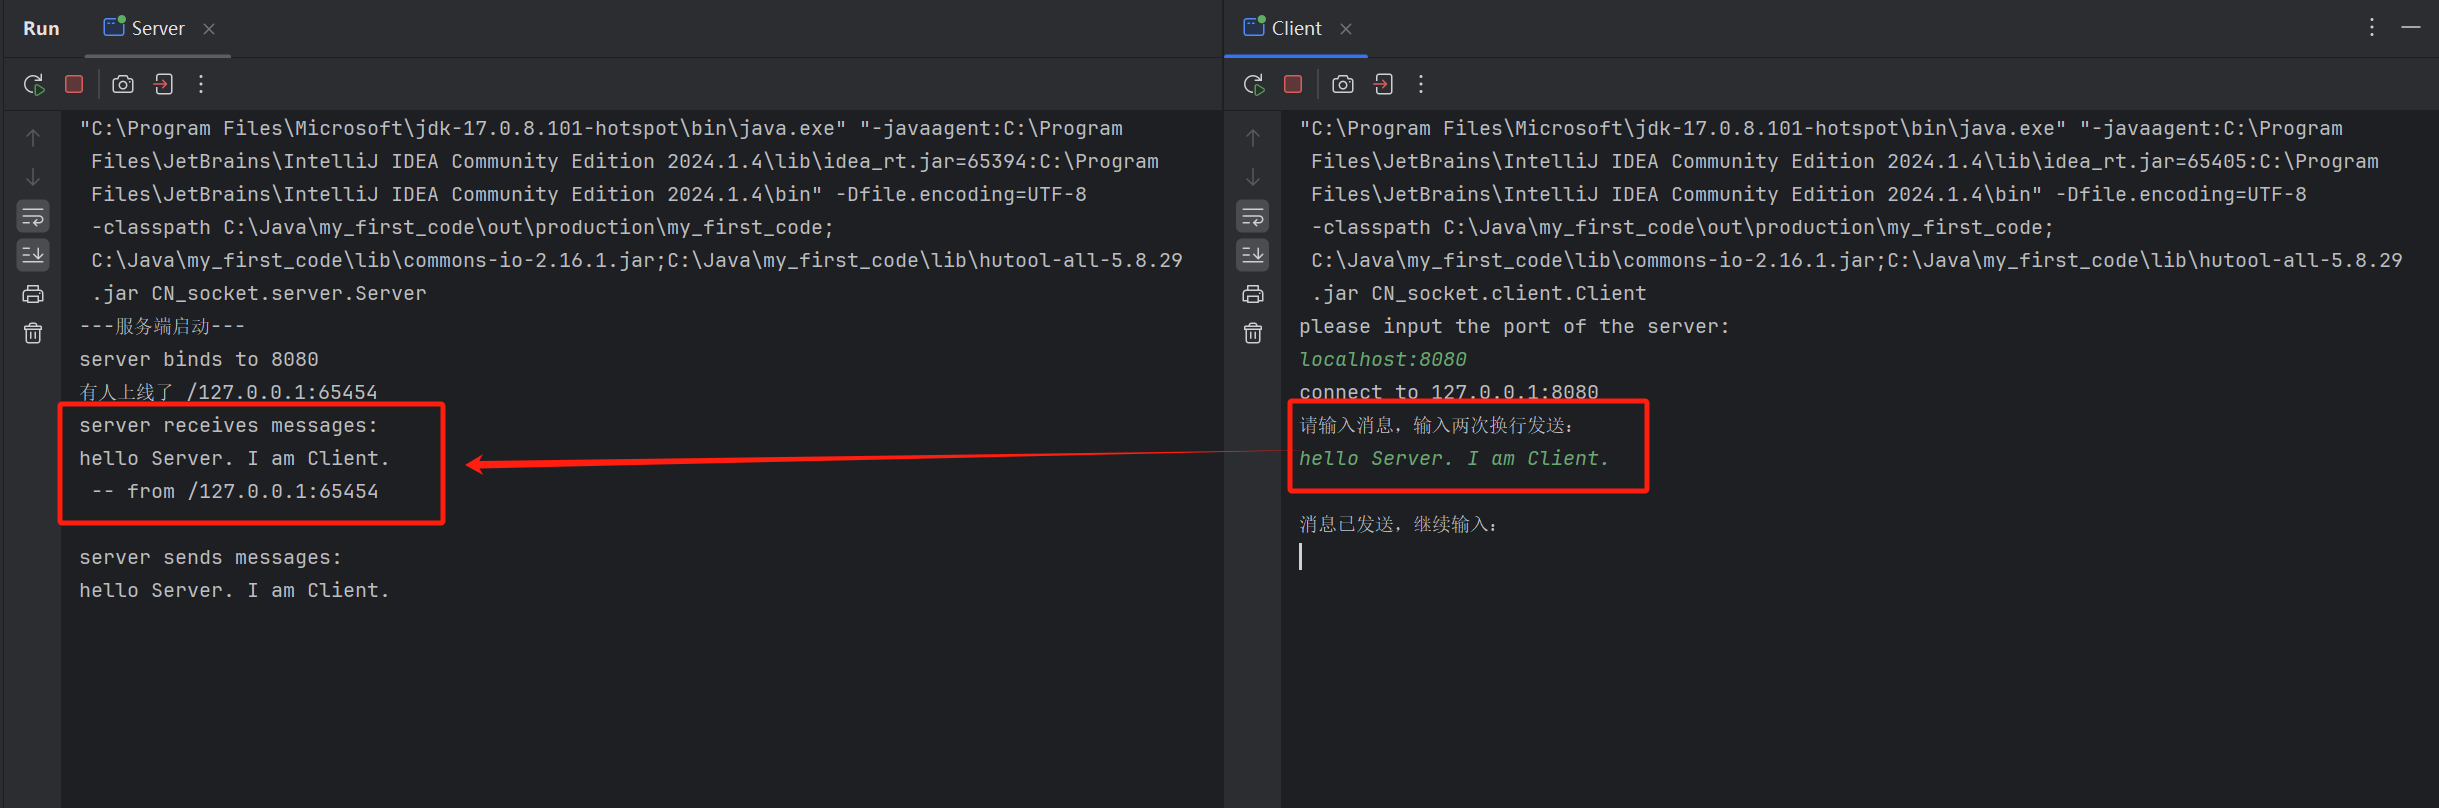
\includegraphics[width=15cm]{./images/1.能在标准输出打印客户端发送的消息.png}
		\caption{能在标准输出打印客户端发送的消息}
	\end{figure}
	
	备注:左(Server)和右(Client)
	
	\subsubsection{支持5个以上客户端同时发送消息并正确打印}
	
	为了满足高并发环境下的服务需求,服务器采用多线程编程模型。每个客户端的连接都由一个独立的线程来处理,这样,即使有多个客户端同时发送消息,服务器也能够并行处理这些请求,确保每个客户端的消息都能被及时接收和正确打印。多线程的使用显著提升了服务器的并发处理能力,增强了系统的实时性和稳定性,从而为用户提供了更加流畅和可靠的服务体验。
	
	\begin{lstlisting}[language=Java, title=支持5个以上客户端同时发送消息并正确打印, tabsize=4]
	// Server.java
	while (true) {
		Socket socket = serverSocket.accept();
		synchronized (onLineSockets) {
			onLineSockets.add(socket);
		}
		System.out.println("有人上线了 " + socket.getRemoteSocketAddress());
		new ServerReaderThread(socket).start();
	}
	\end{lstlisting}
	
	此处我使用六个Client和一个Server作为测试,测试结果如下图所示:
	
	首先展示的是Server的实验结果:
	
	\begin{figure}[H]
		\centering
		\begin{minipage}[b]{0.45\textwidth}
			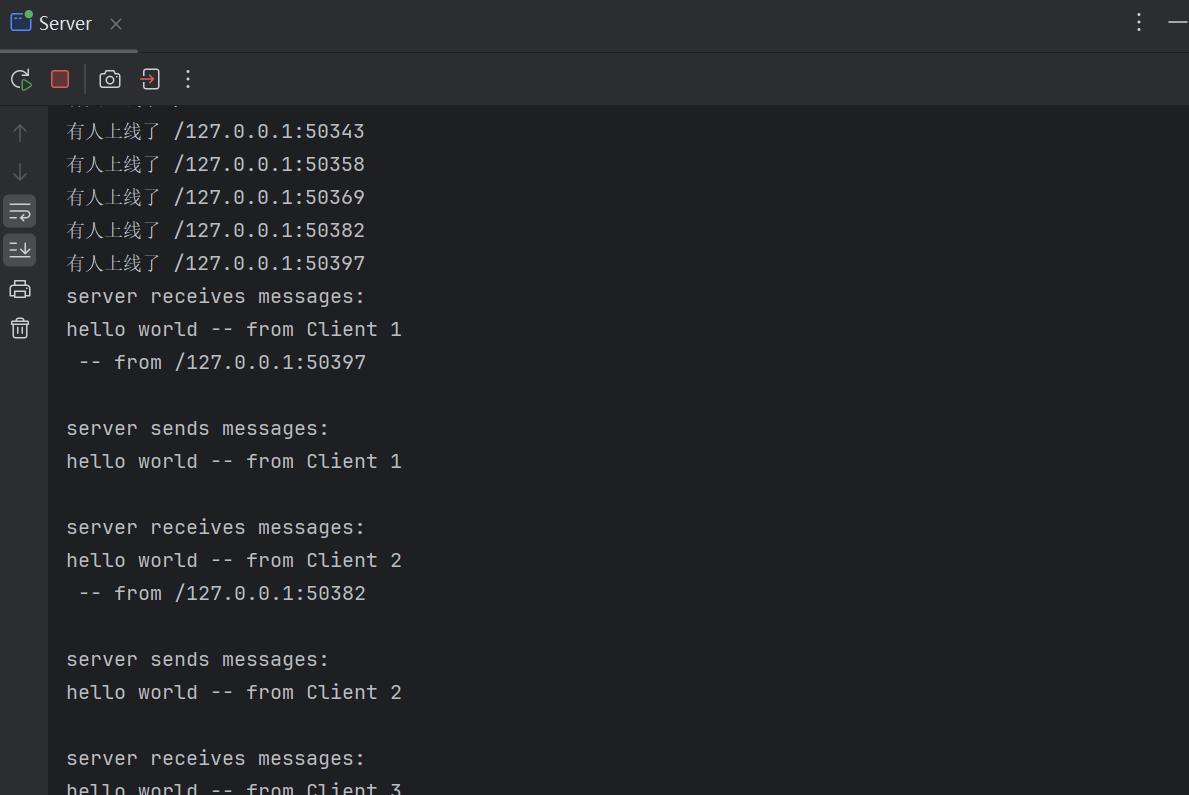
\includegraphics[width=\textwidth]{./images/2.支持5个以上客户端同时发送消息并逐一打印-Server-1.png}
			\caption{Server-1}
		\end{minipage}
		\hfill
		\begin{minipage}[b]{0.45\textwidth}
			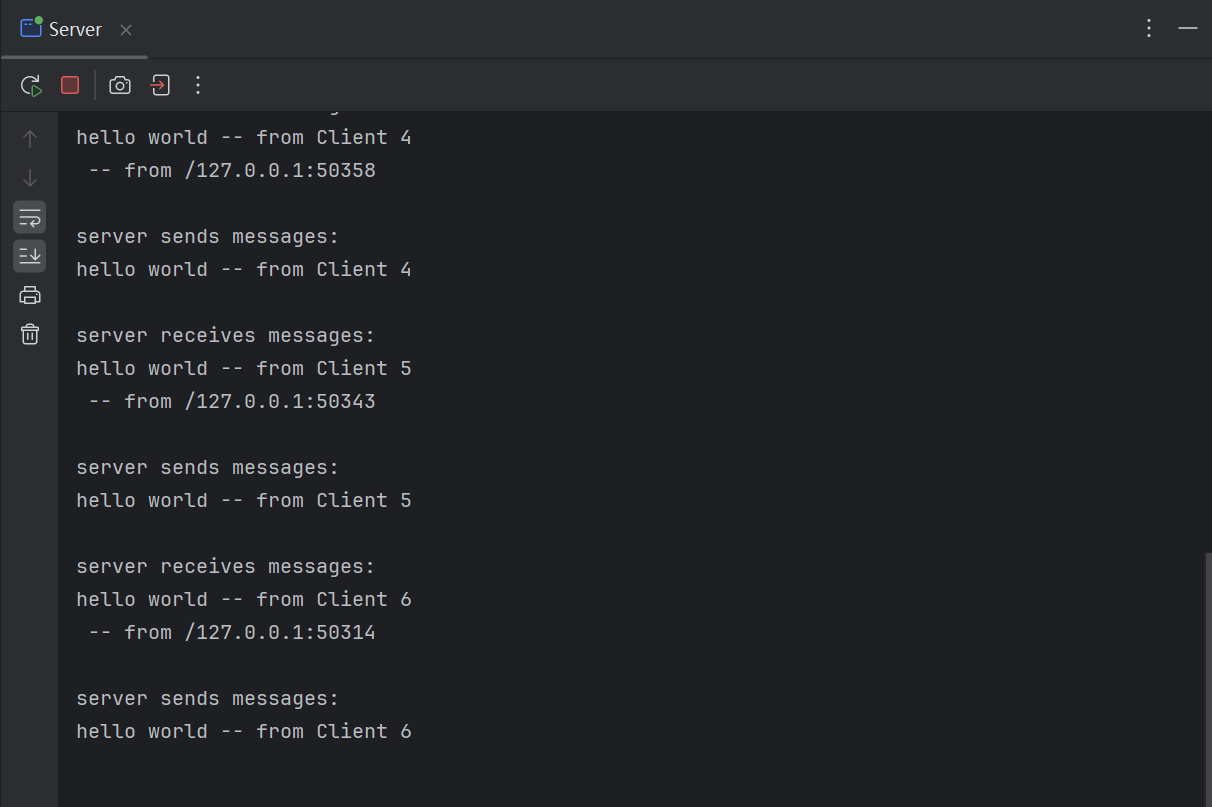
\includegraphics[width=\textwidth]{./images/2.支持5个以上客户端同时发送消息并逐一打印-Server-2.png}
			\caption{Server-2}
		\end{minipage}
	\end{figure}
	
	通过测试发现,Server发送的消息只会被其中一个Client收到,所以我的想法是在程序中设置一个记录在线的客户端的List,取名为onLineSockets,在发消息的时候遍历onLineSockets即可。
	
	\begin{lstlisting}[language=Java, title=完善-支持5个以上客户端同时发送消息并正确打印, tabsize=4]
	// Server.java
	public static List<Socket> onLineSockets = new ArrayList<>();
	// 广播消息给所有在线客户端
	public static void broadcastMessage(String message) {
		synchronized (onLineSockets) {
			for (Socket socket : onLineSockets) {
				try {
					DataOutputStream dos = new DataOutputStream(socket.getOutputStream());
					dos.writeUTF(message);
					dos.flush();
				} catch (Exception e) {
					System.out.println("消息发送失败:" + socket.getRemoteSocketAddress());
				}
			}
		}
	}
	\end{lstlisting}
	
	这样一来也解决了只有一个客户端收到消息的问题。
	
	以下是六个Client的实验结果:
	
	\begin{figure}[H]
		\centering
		\begin{minipage}[b]{0.45\textwidth}
			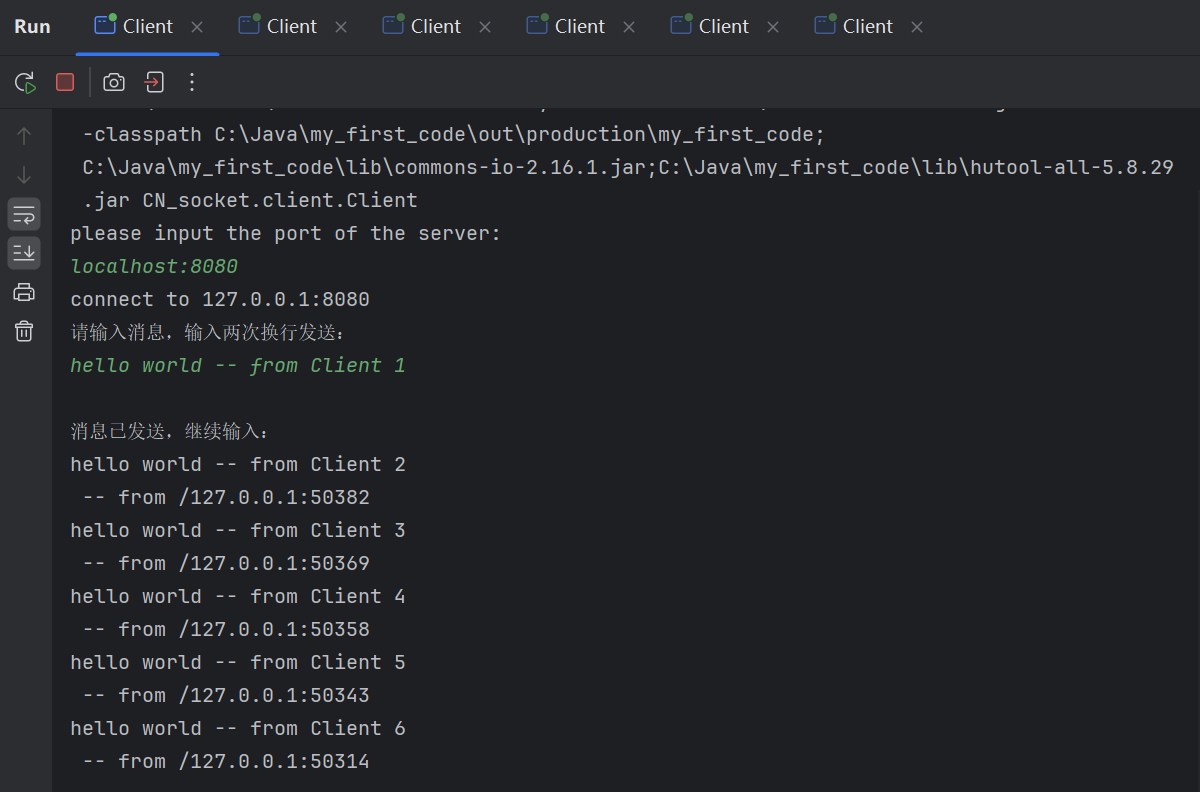
\includegraphics[width=\textwidth]{./images/2.支持5个以上客户端同时发送消息并逐一打印-Client1.png}
			\caption{Client-1}
		\end{minipage}
		\hfill
		\begin{minipage}[b]{0.45\textwidth}
			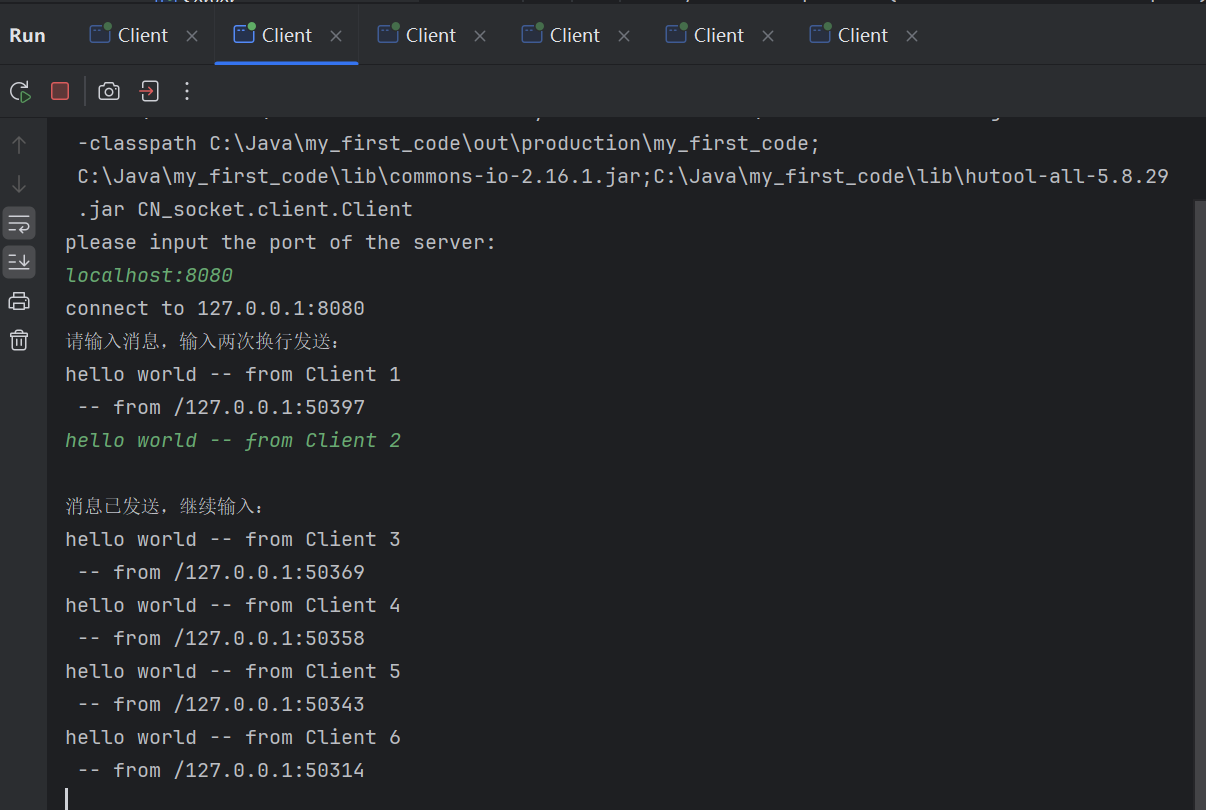
\includegraphics[width=\textwidth]{./images/2.支持5个以上客户端同时发送消息并逐一打印-Client2.png}
			\caption{Client-2}
		\end{minipage}
	\end{figure}
	
	\begin{figure}[H]
		\centering
		\begin{minipage}[b]{0.45\textwidth}
			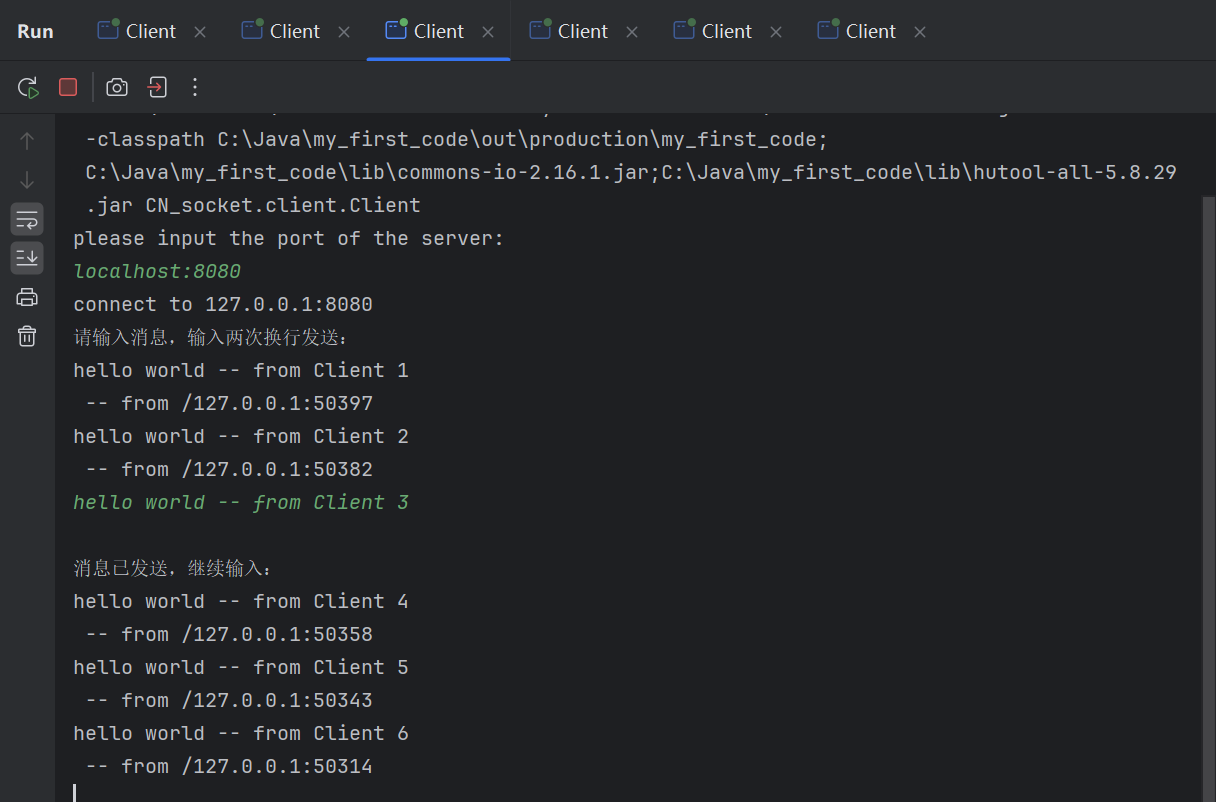
\includegraphics[width=\textwidth]{./images/2.支持5个以上客户端同时发送消息并逐一打印-Client3.png}
			\caption{Client-3}
		\end{minipage}
		\hfill
		\begin{minipage}[b]{0.45\textwidth}
			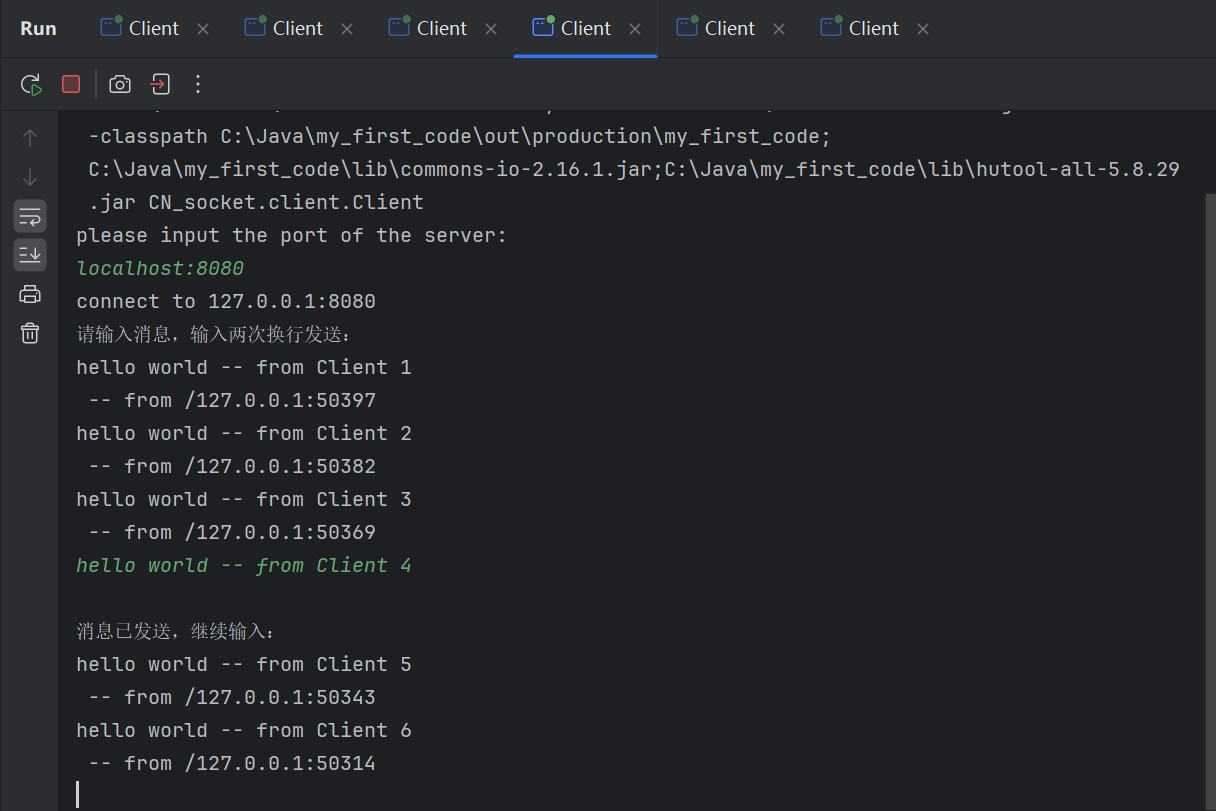
\includegraphics[width=\textwidth]{./images/2.支持5个以上客户端同时发送消息并逐一打印-Client4.png}
			\caption{Client-4}
		\end{minipage}
	\end{figure}
	
	\begin{figure}[H]
		\centering
		\begin{minipage}[b]{0.45\textwidth}
			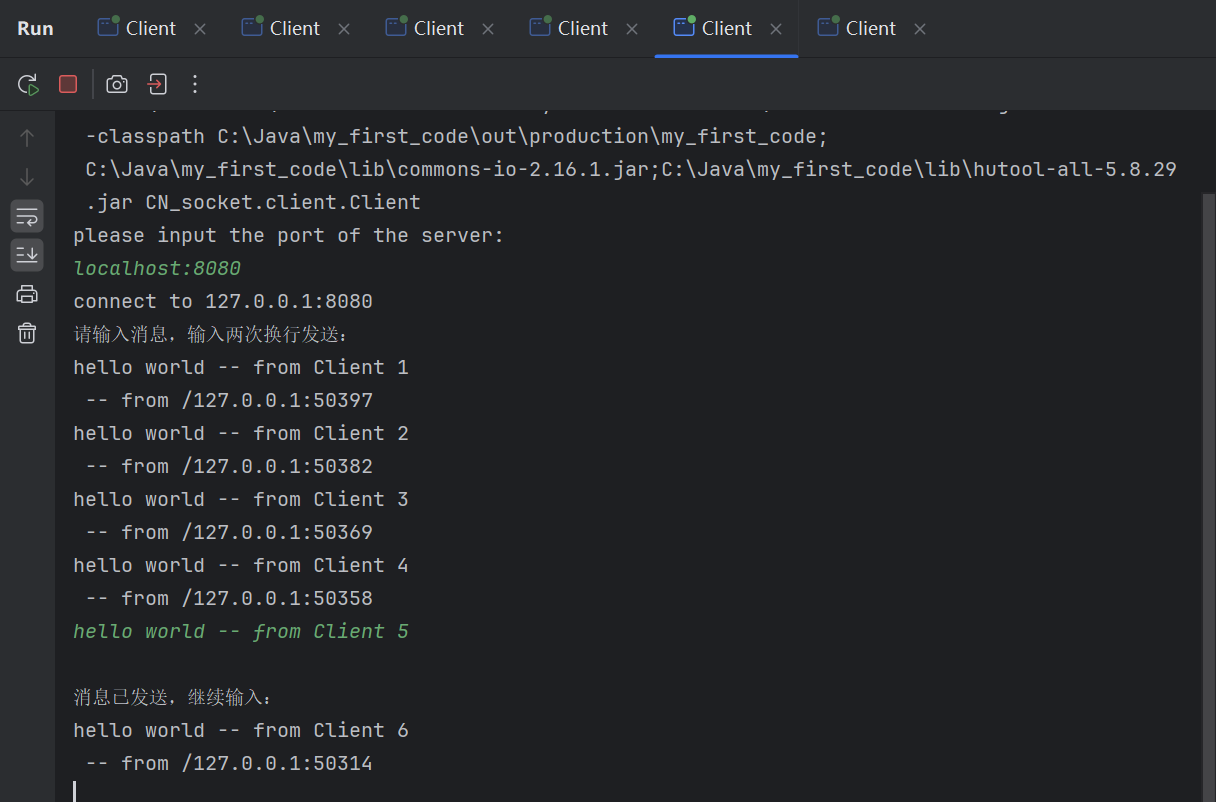
\includegraphics[width=\textwidth]{./images/2.支持5个以上客户端同时发送消息并逐一打印-Client5.png}
			\caption{Client-5}
		\end{minipage}
		\hfill
		\begin{minipage}[b]{0.45\textwidth}
			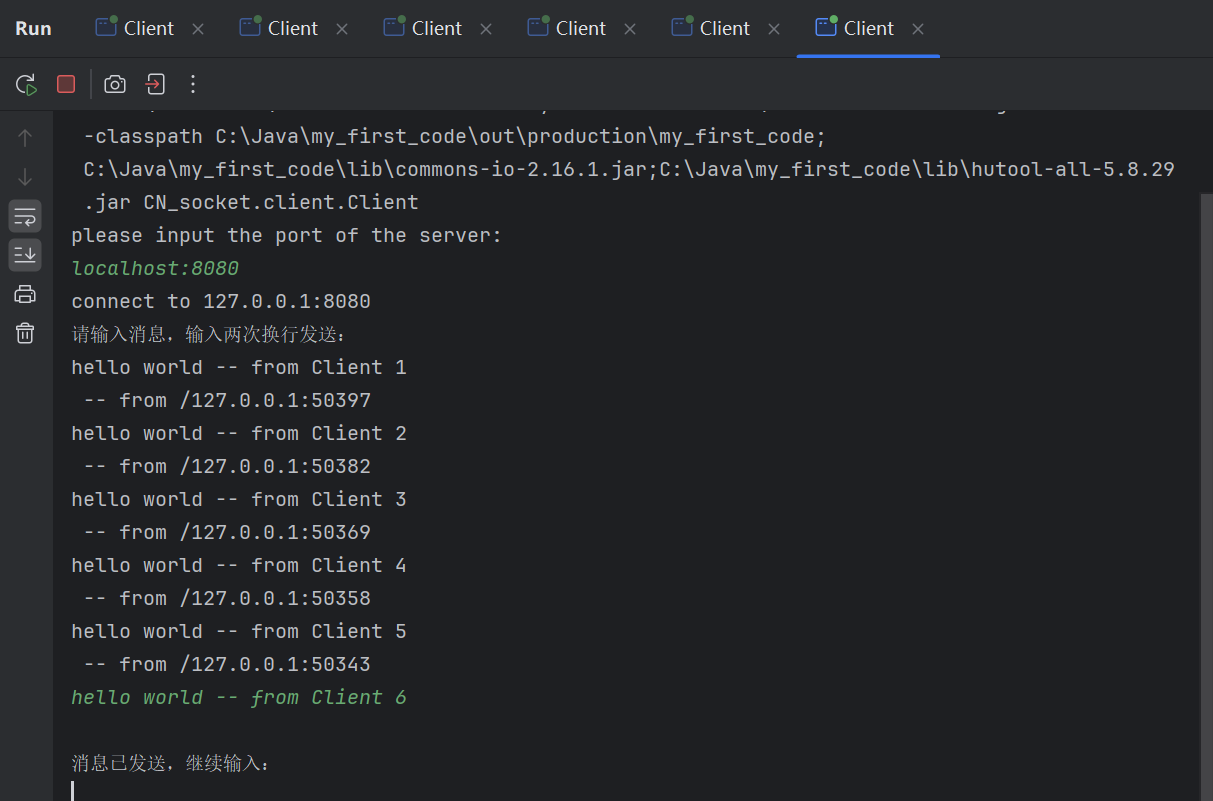
\includegraphics[width=\textwidth]{./images/2.支持5个以上客户端同时发送消息并逐一打印-Client6.png}
			\caption{Client-6}
		\end{minipage}
	\end{figure}
	
	\subsubsection{绑定至错误的端口号时能提示出错信息}
	
	在服务器初始化过程中,对指定的端口号进行有效性检查是至关重要的。如果端口号不在合法范围内(通常为0-65535),或者该端口已被其他服务占用,服务器在尝试绑定时将无法成功。此时,系统应捕获相应的异常,并给出明确的错误提示信息,指导用户采取正确的操作。这不仅提升了用户体验,也有助于快速定位和解决问题。
	
	\begin{lstlisting}[language=Java, title=绑定至错误的端口号时能提示出错信息, tabsize=4]
	// Client.java
	try {
		// address 是用户输入的 IP 地址,port_ 是用户输入的端口号
		if (port_ > 0 && port_ < 65535) {
			port = port_;
			
			// 创建 Socket 对象,请求连接到指定服务器
			Socket socket = new Socket(address, port);
			
			// 创建一个独立的线程,用于接收服务器发送的消息
			new ClientReaderThread(socket).start();
		}
	} catch (IllegalArgumentException e) {
		System.err.println("Wrong input: " + e.getMessage());
	} catch (Exception e) {
		e.printStackTrace();
	}
	\end{lstlisting}
	
	测试结果如下:
	
	\begin{figure}[H]
		\centering
		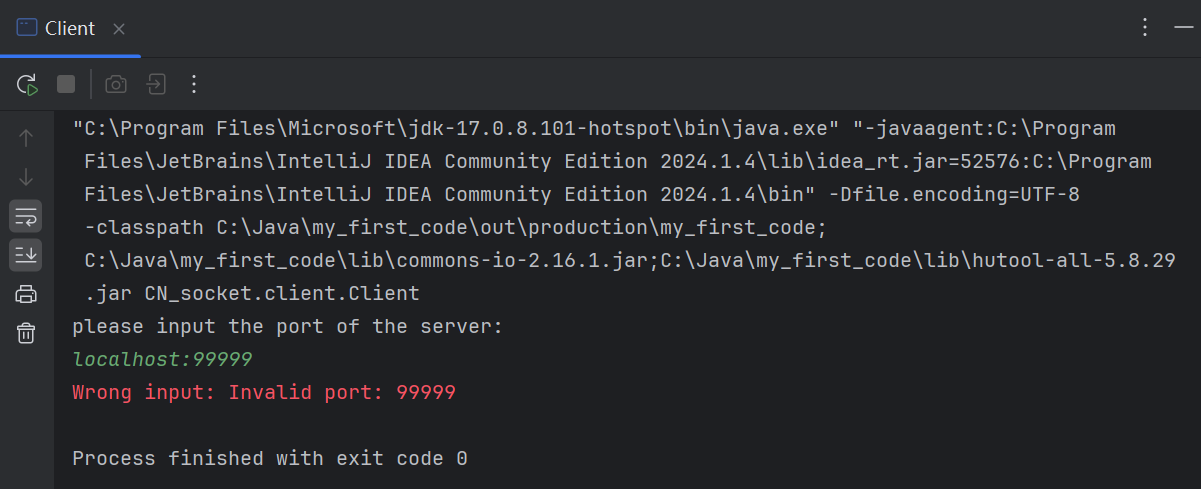
\includegraphics[width=11cm]{./images/3.绑定至错误的端口号时提示出错信息-1.png}
		\caption{绑定至过大(大于65535)的端口号时提示出错信息}
	\end{figure}
	
	\begin{figure}[H]
		\centering
		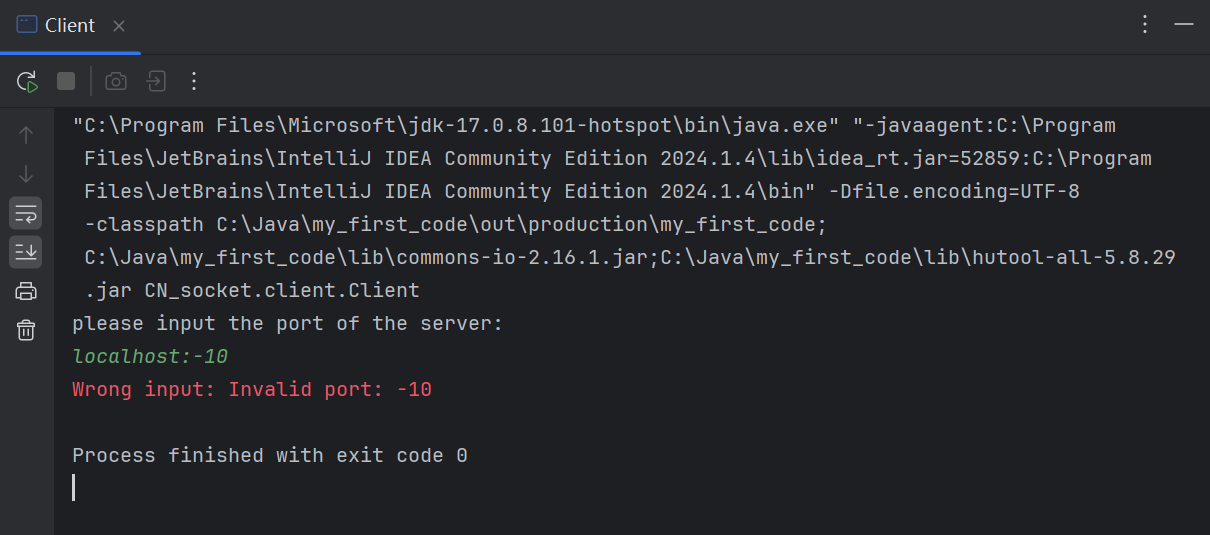
\includegraphics[width=11cm]{./images/3.绑定至错误的端口号时提示出错信息-2.png}
		\caption{绑定至过小(小于0)的端口号时提示出错信息}
	\end{figure}
	
	\subsection{Client}
	
	\subsubsection{能从标准输入或文件接收消息}
	
	设计一个线程,专门用于读取socket输入流中的数据,使用Socket和DataInputStream来实现这一功能
	
	\begin{lstlisting}[language=Java, title=能从标准输入或文件接收消息, tabsize=4]
	// ClientReaderThread.java
	InputStream is = socket.getInputStream();
	DataInputStream dis = new DataInputStream(is);
	String message = dis.readUTF();
	System.out.println(message);
	\end{lstlisting}
	
	\begin{figure}[H]
		\centering
		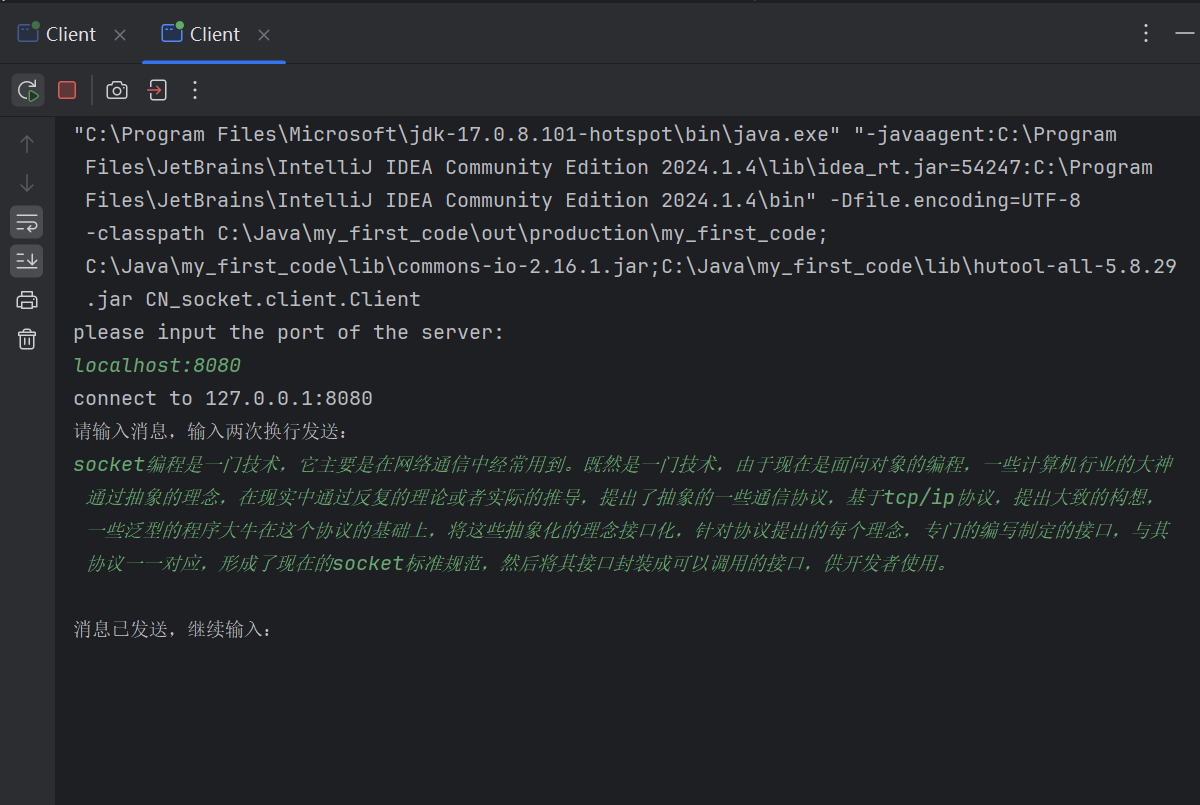
\includegraphics[width=11cm]{./images/4.能从标准输入或文件接收信息-Client1.png}
		\caption{能从标准输入或文件接收信息(第一个Client-用于发送消息)}
	\end{figure}
	
	\begin{figure}[H]
		\centering
		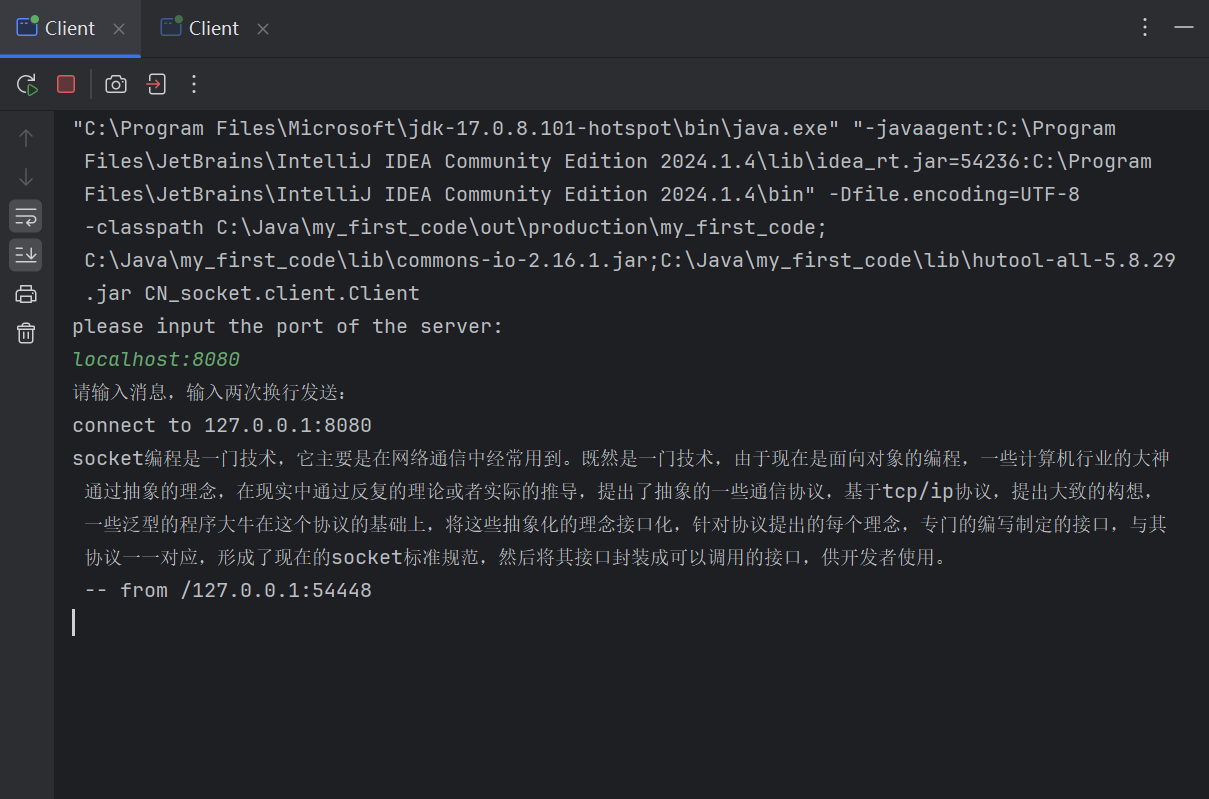
\includegraphics[width=11cm]{./images/4.能从标准输入或文件接收信息-Client2.png}
		\caption{能从标准输入或文件接收信息(第二个Client-用于接收消息)}
	\end{figure}
	
	\begin{figure}[H]
		\centering
		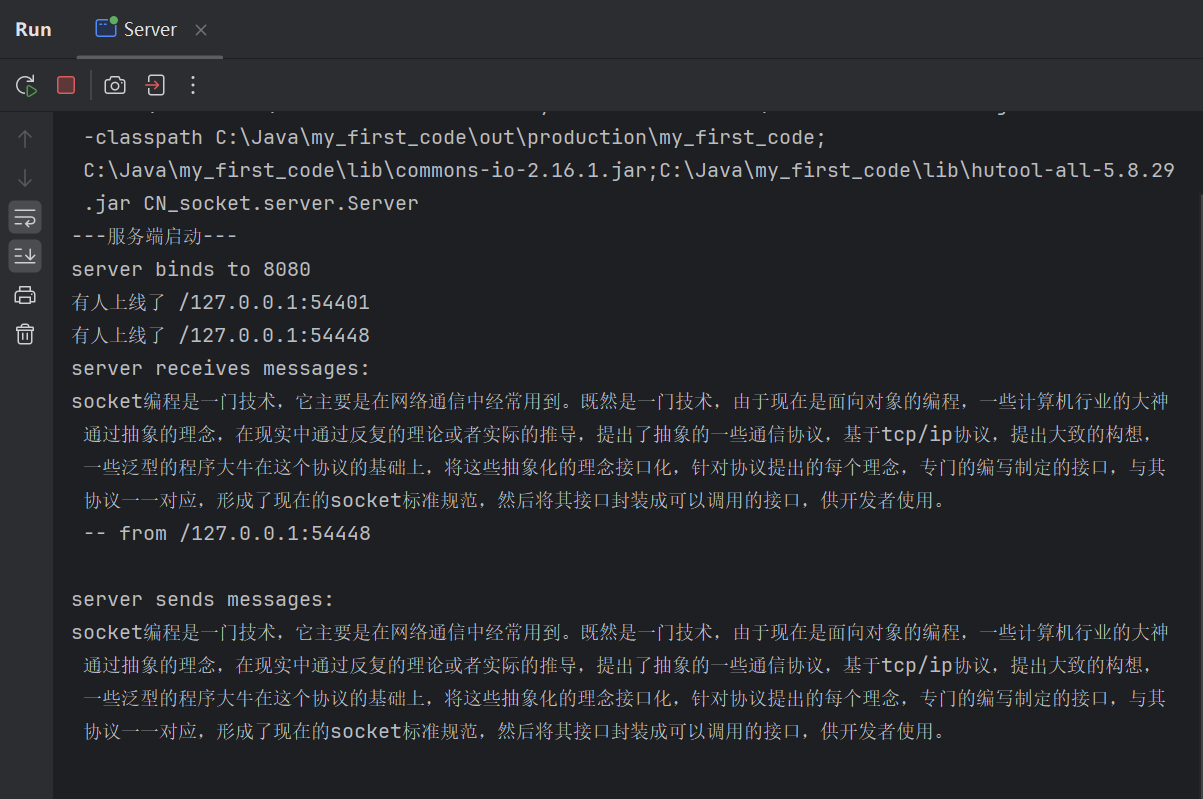
\includegraphics[width=11cm]{./images/4.能从标准输入或文件接收信息-Server.png}
		\caption{能从标准输入或文件接收信息(Server端)}
	\end{figure}
	
	\subsubsection{标准输入消息以两次回车作为结束标志}
	
	每次循环读取一行输入,并将这些行累积到一个字符串中。当用户输入两次回车时,认为这是消息结束的信号。此时,程序将停止读取输入,并将累积的消息发送到服务器。
	
	\begin{lstlisting}[language=Java, title=标准输入消息以两次回车作为结束标志, tabsize=4]
	// Client.java
	// 用户输入消息并发送到服务器
	Scanner scanner = new Scanner(System.in);
	System.out.println("请输入消息,输入两次换行发送:");
	StringBuilder messageBuilder = new StringBuilder();
	while (true) {
		String line = scanner.nextLine();
		if (line.isEmpty()) {
			// 检测到双换行,发送消息
			String message = messageBuilder.toString();
			if (message.trim().isEmpty()) {
				System.out.println("欢迎下次使用!退出成功");
				dos.close();
				socket.close();
				break;
			}
			dos.writeUTF(message); // 发送消息
			dos.flush(); // 刷新输出流
			messageBuilder.setLength(0); // 清空缓冲区
			System.out.println("消息已发送,继续输入:");
		} else {
			// 累积消息内容
			messageBuilder.append(line).append("\n");
		}
	}
	\end{lstlisting}
	
	测试结果如下:
	
	在Client端口通过两次回车来确认发送:
	
	\begin{figure}[H]
		\centering
		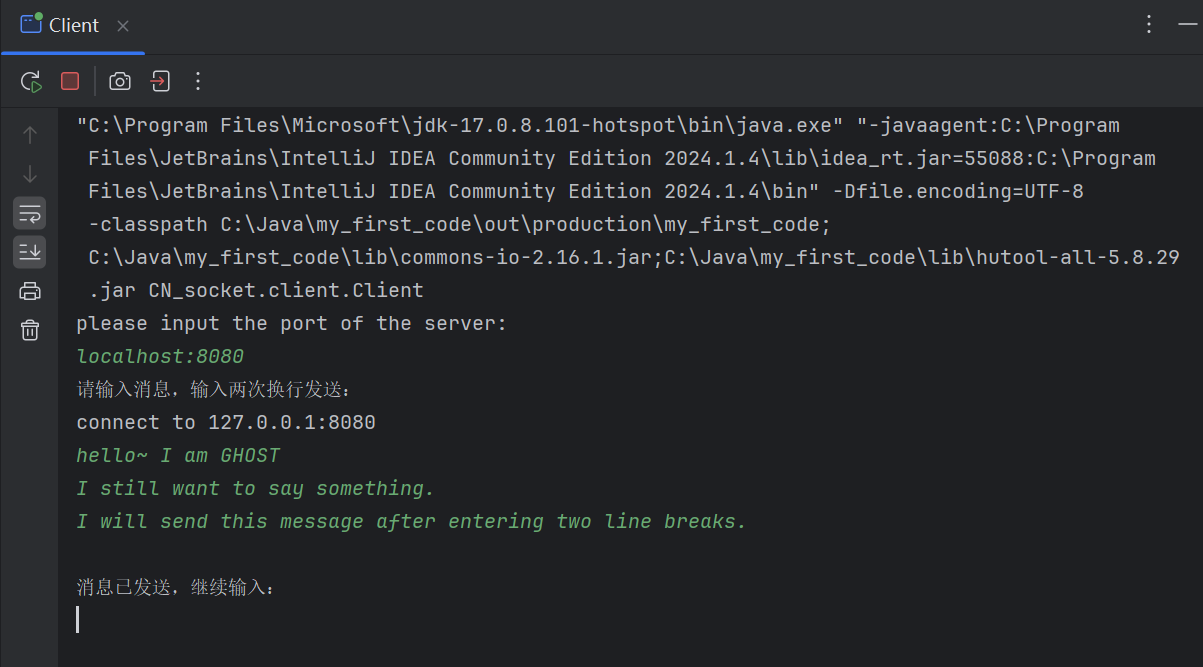
\includegraphics[width=11cm]{./images/5.标准输入信息以两次回车作为结束标志-Client.png}
		\caption{标准输入信息以两次回车作为结束标志(Client端发送)}
	\end{figure}
	
	在Server端可以接收到Client确认发送出来的消息
	
	\begin{figure}[H]
		\centering
		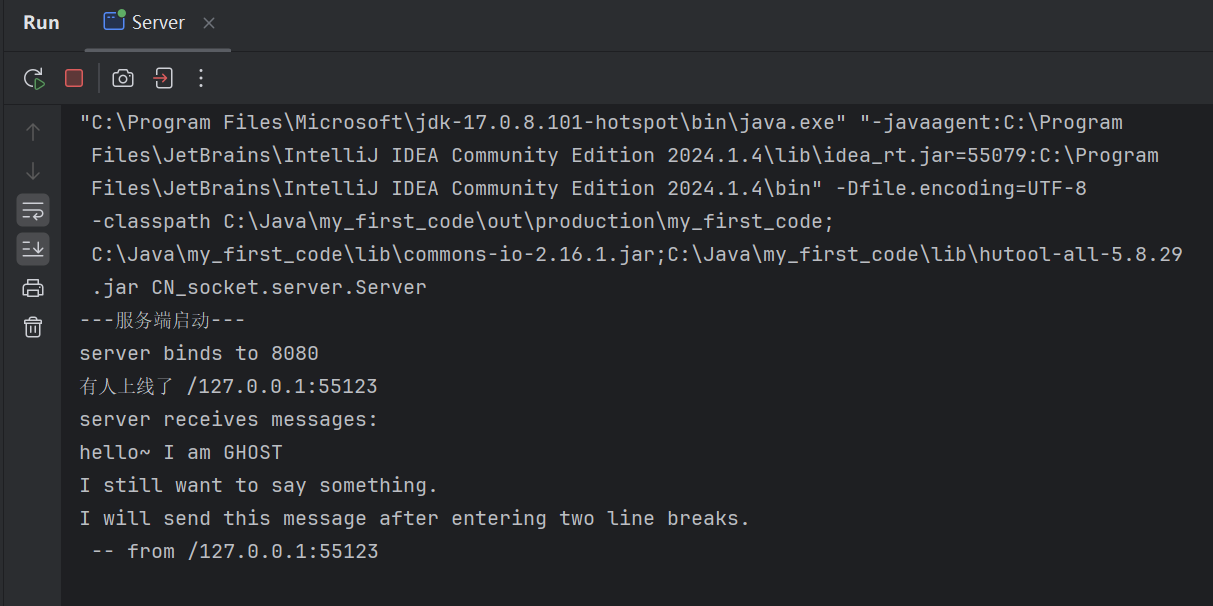
\includegraphics[width=11cm]{./images/5.标准输入信息以两次回车作为结束标志-Server.png}
		\caption{标准输入信息以两次回车作为结束标志(Server端接收)}
	\end{figure}
	
	\subsubsection{连接至错误的IP地址/端口号时能提示出错信息}
	
	添加逻辑来验证IP地址是否符合标准的格式,以及端口号是否在合法的范围内即可。如果检查失败,程序将不会尝试建立连接,而是立即向用户显示一个错误消息,说明问题所在。
	
	这里将IP和端口号连接错误的报错信息分开处理,可以更好的将结果展现给用户。
	
	\begin{lstlisting}[language=Java, title=连接至错误的IP地址/端口号时能提示出错信息, tabsize=4]
	// Client.java
	// 提示用户输入服务器地址和端口号
	System.out.println("please input the port of the server: ");
	String address_ = sc.nextLine();
	String address = address_.split(":")[0];
	int port_ = Integer.parseInt(address_.split(":")[1]);
	int port = 0;
	
	try {
		
		···
		
		} else {
			throw new IllegalArgumentException("Invalid port: " + port_);
		}
	} catch (IllegalArgumentException e) {
		System.err.println("Wrong input: " + e.getMessage());
	} catch (Exception e) {
		e.printStackTrace();
	}
	\end{lstlisting}
	
	首先测试连接至错误的IP的时候的错误提示,这里将IP写为:128.0.0.1:
	
	\begin{figure}[H]
		\centering
		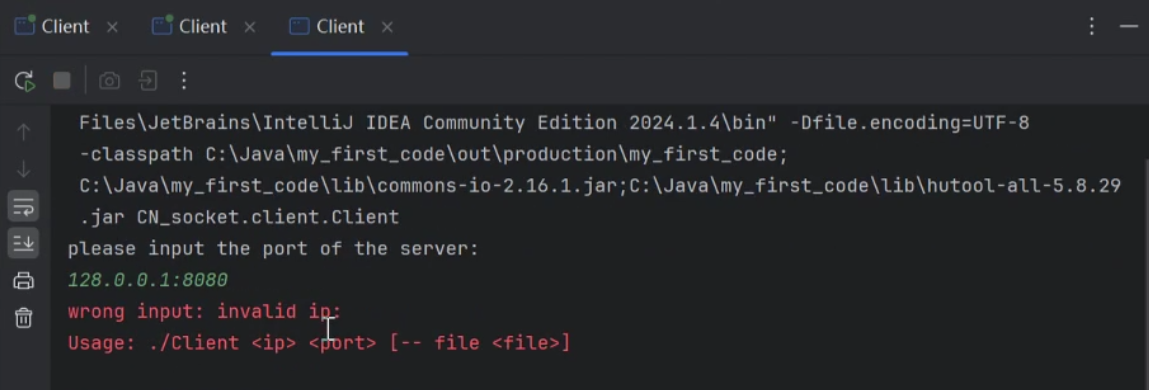
\includegraphics[width=11cm]{./images/6.连接至错误的IP地址时能提示错误信息.png}
		\caption{连接至错误的IP地址时能提示错误信息}
	\end{figure}
	
	再来测试输入错误的端口号时的错误提示,这里输入8090作为错误的端口号:
	
	\begin{figure}[H]
		\centering
		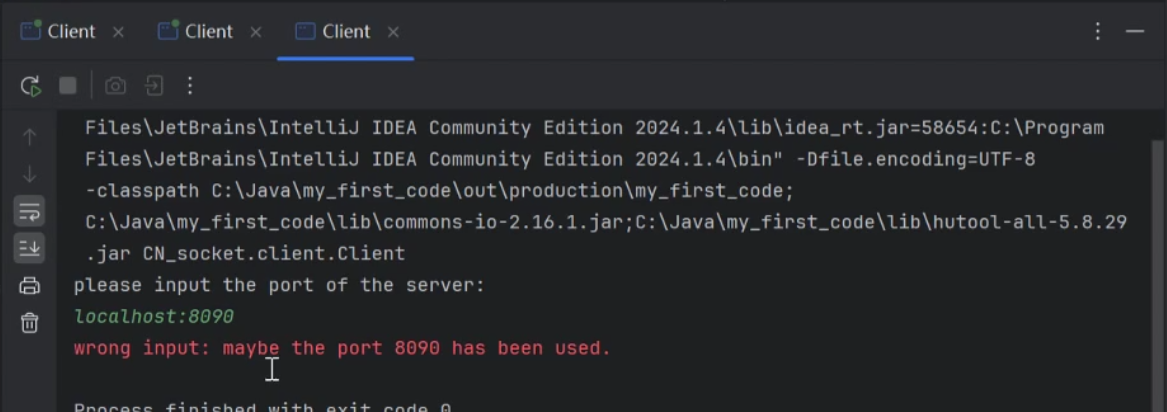
\includegraphics[width=11cm]{./images/6.连接至错误的端口号时能提示错误信息.png}
		\caption{连接至错误的端口号时能提示错误信息}
	\end{figure}
	
	\subsection{整体}
	
	\subsubsection{支持在localhost及在两台不同机器上运行}
	
	本次实验中,我采用先在本地打开多个Client来测试localhost的可用性,再在两台电脑上完成不同机器的远程连接,并重复前面的步骤来测试本次实验的代码的实现效果。
	
	在localhost的多个终端上测试的结果已经在4.1.2的部分展现,所以此处不再描述。
	
	\vspace{12pt}
	
	以下是我在两台不同机器下运行的结果:(两台电脑都是Windows系统下的机器)
	
	\begin{figure}[H]
		\centering
		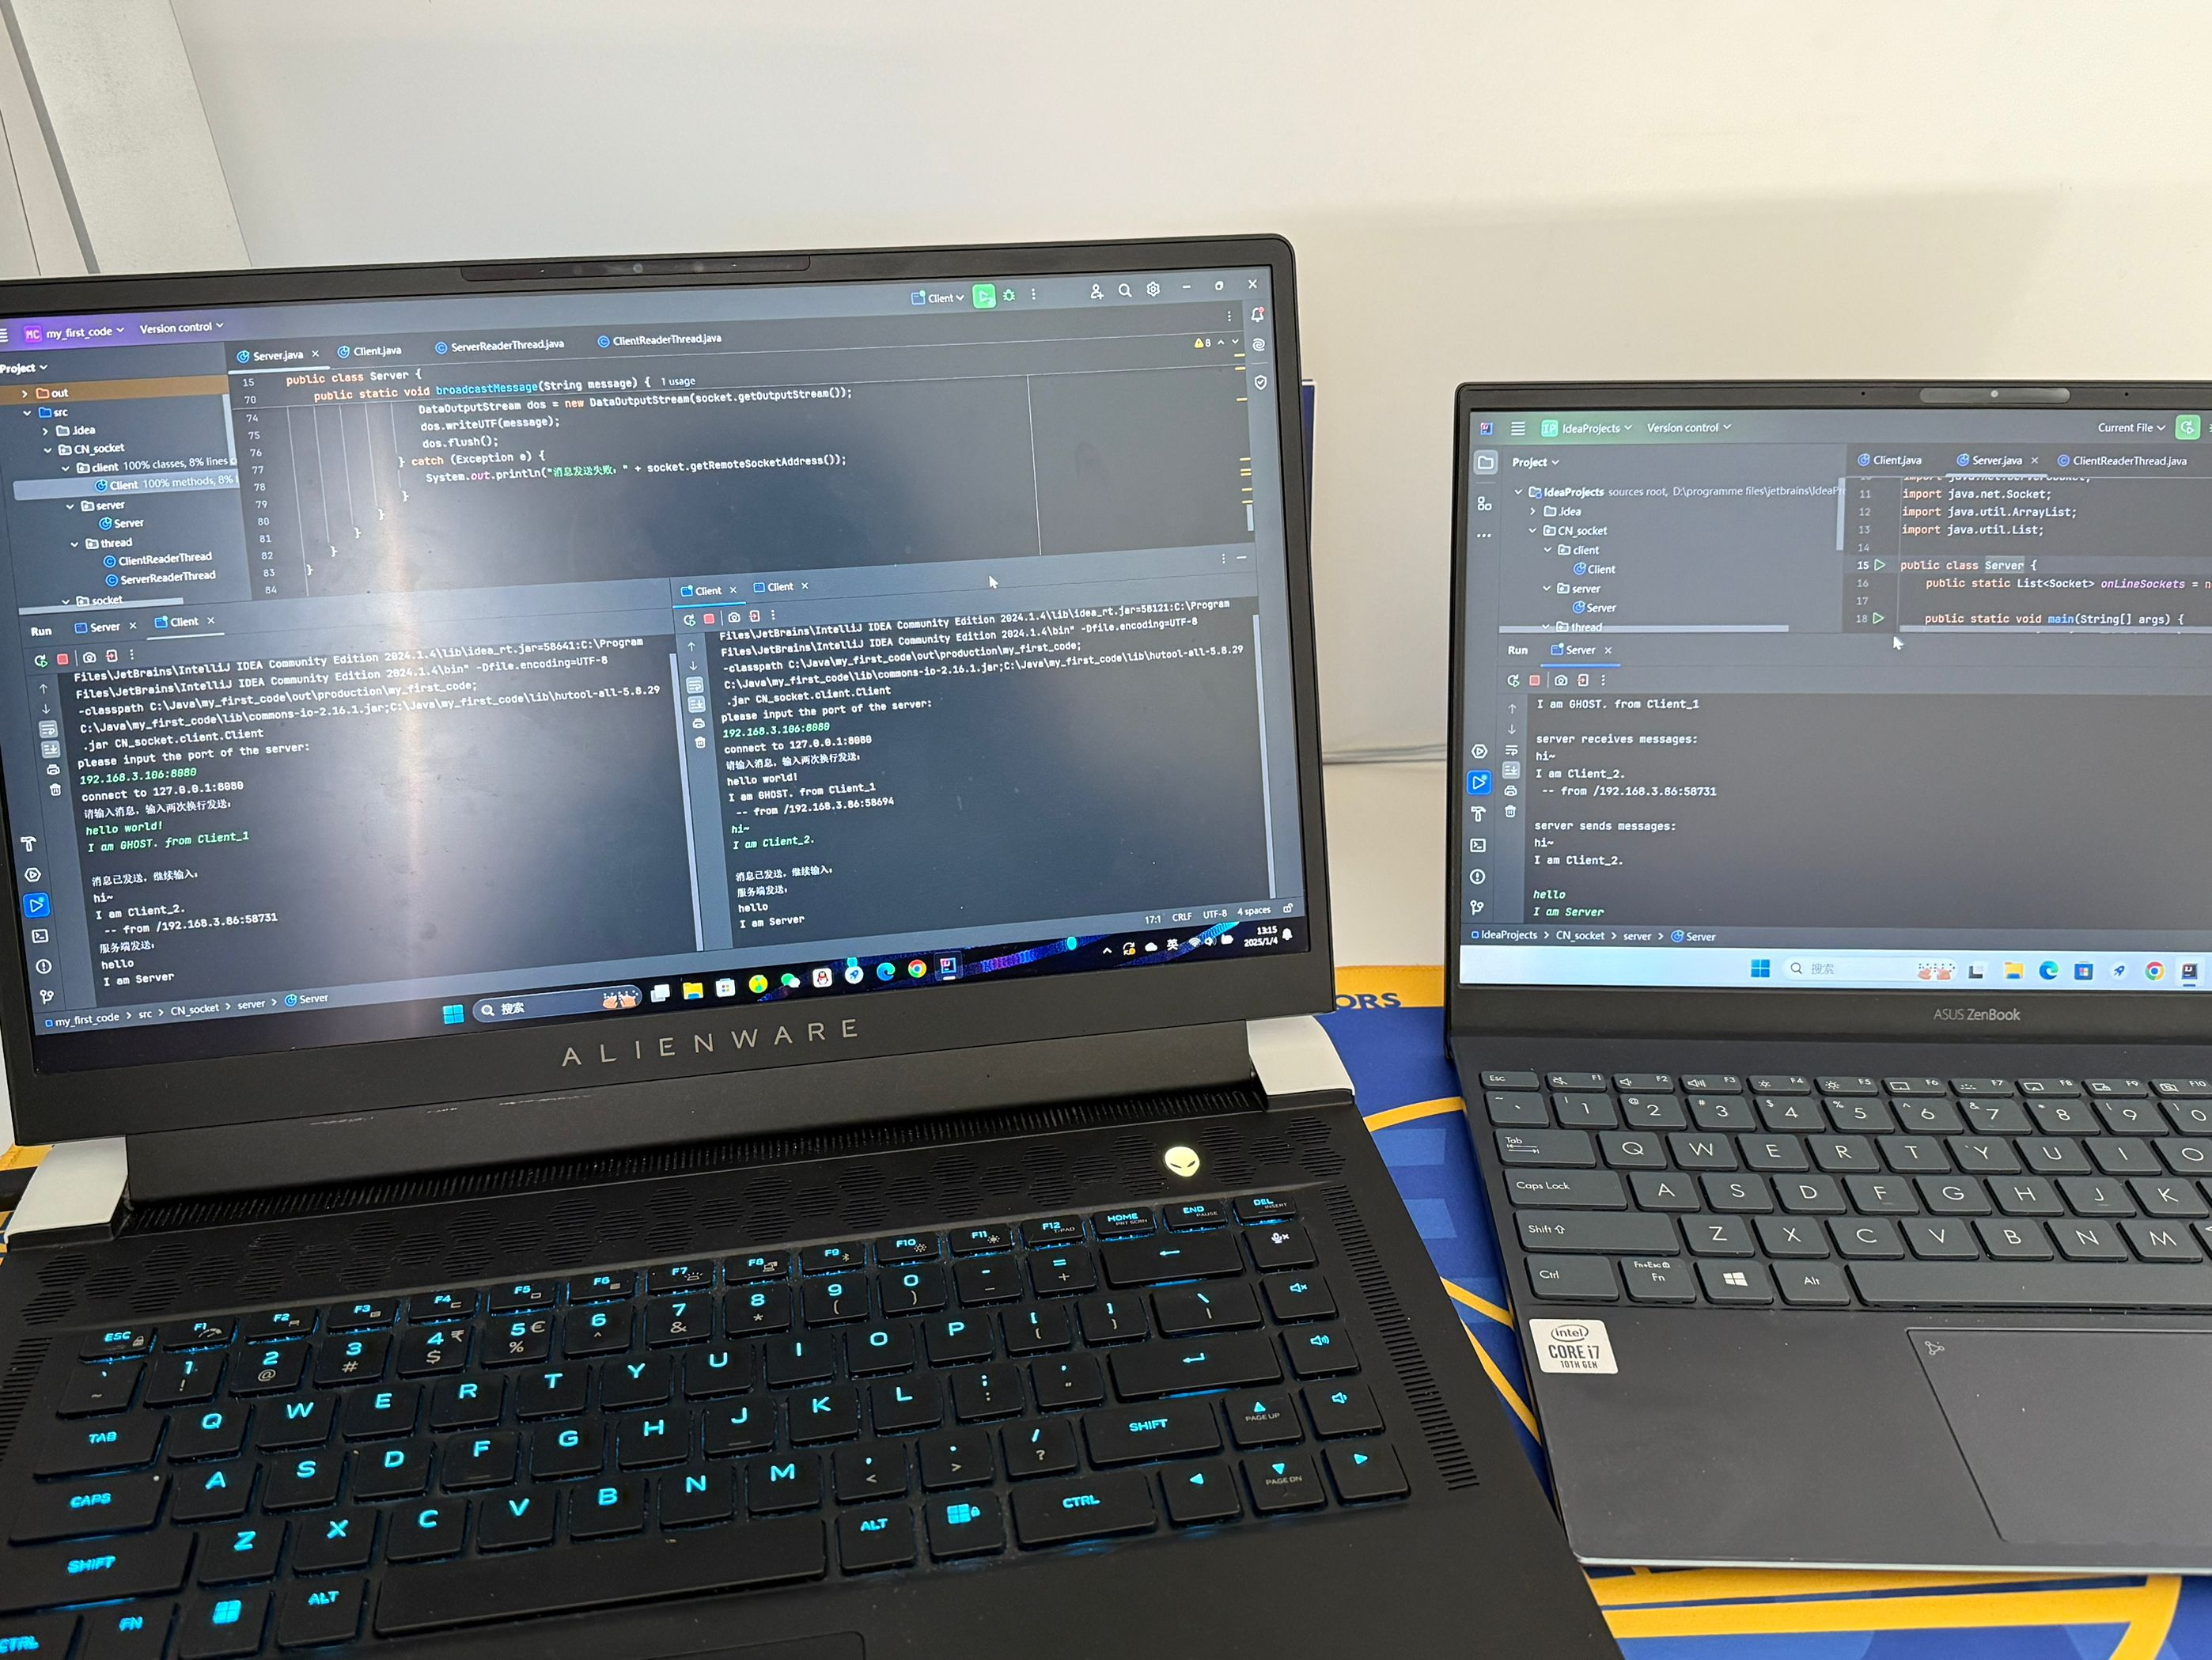
\includegraphics[width=11cm]{./images/7.支持在localhost及两台不同机器上运行.jpg}
		\caption{支持在两台不同机器上运行}
	\end{figure}
	
	备注:左边的电脑开启两个终端作为两个Client,右边的电脑作为Server来接收和转发消息:
	
	具体来看一下Client和Server在两台机器下完成的任务:
	
	\begin{figure}[H]
		\centering
		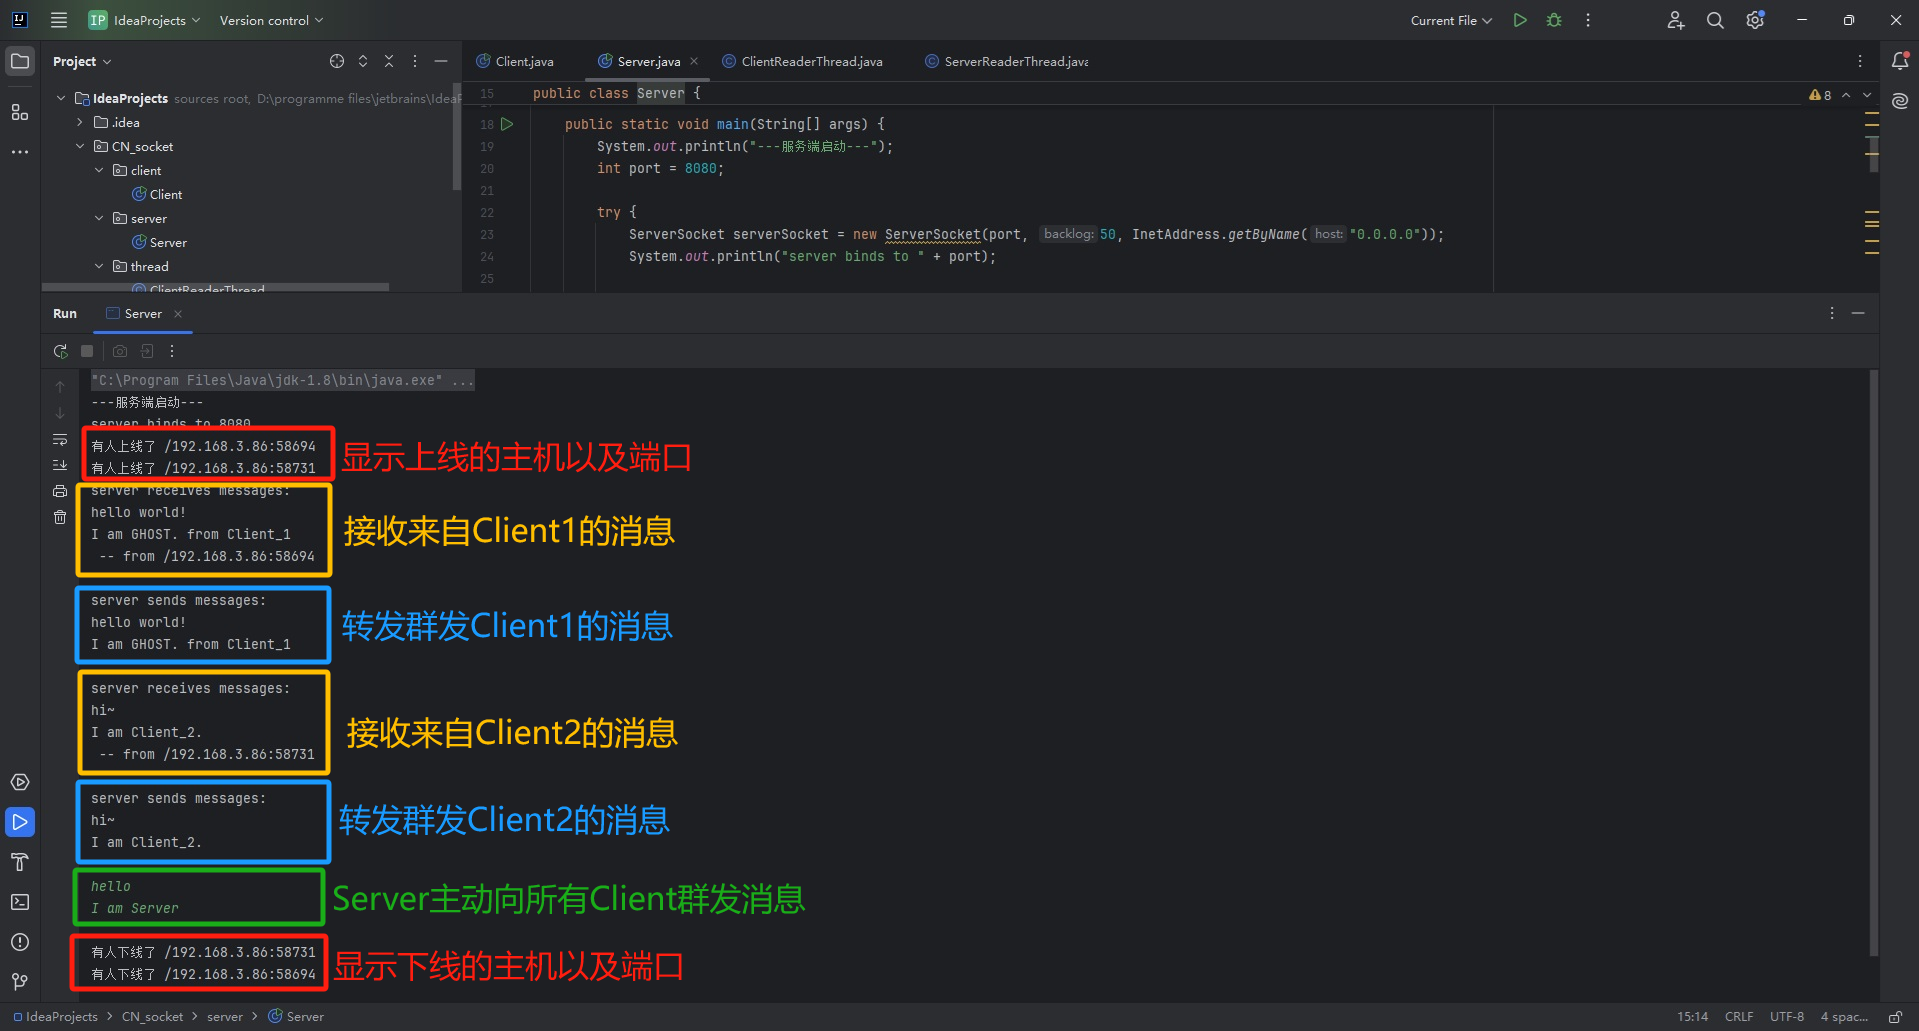
\includegraphics[width=15cm]{./images/7.支持在不同机器上通信-Server端.png}
		\caption{支持在不同机器上通信-Server端}
	\end{figure}
	
	\begin{figure}[H]
		\centering
		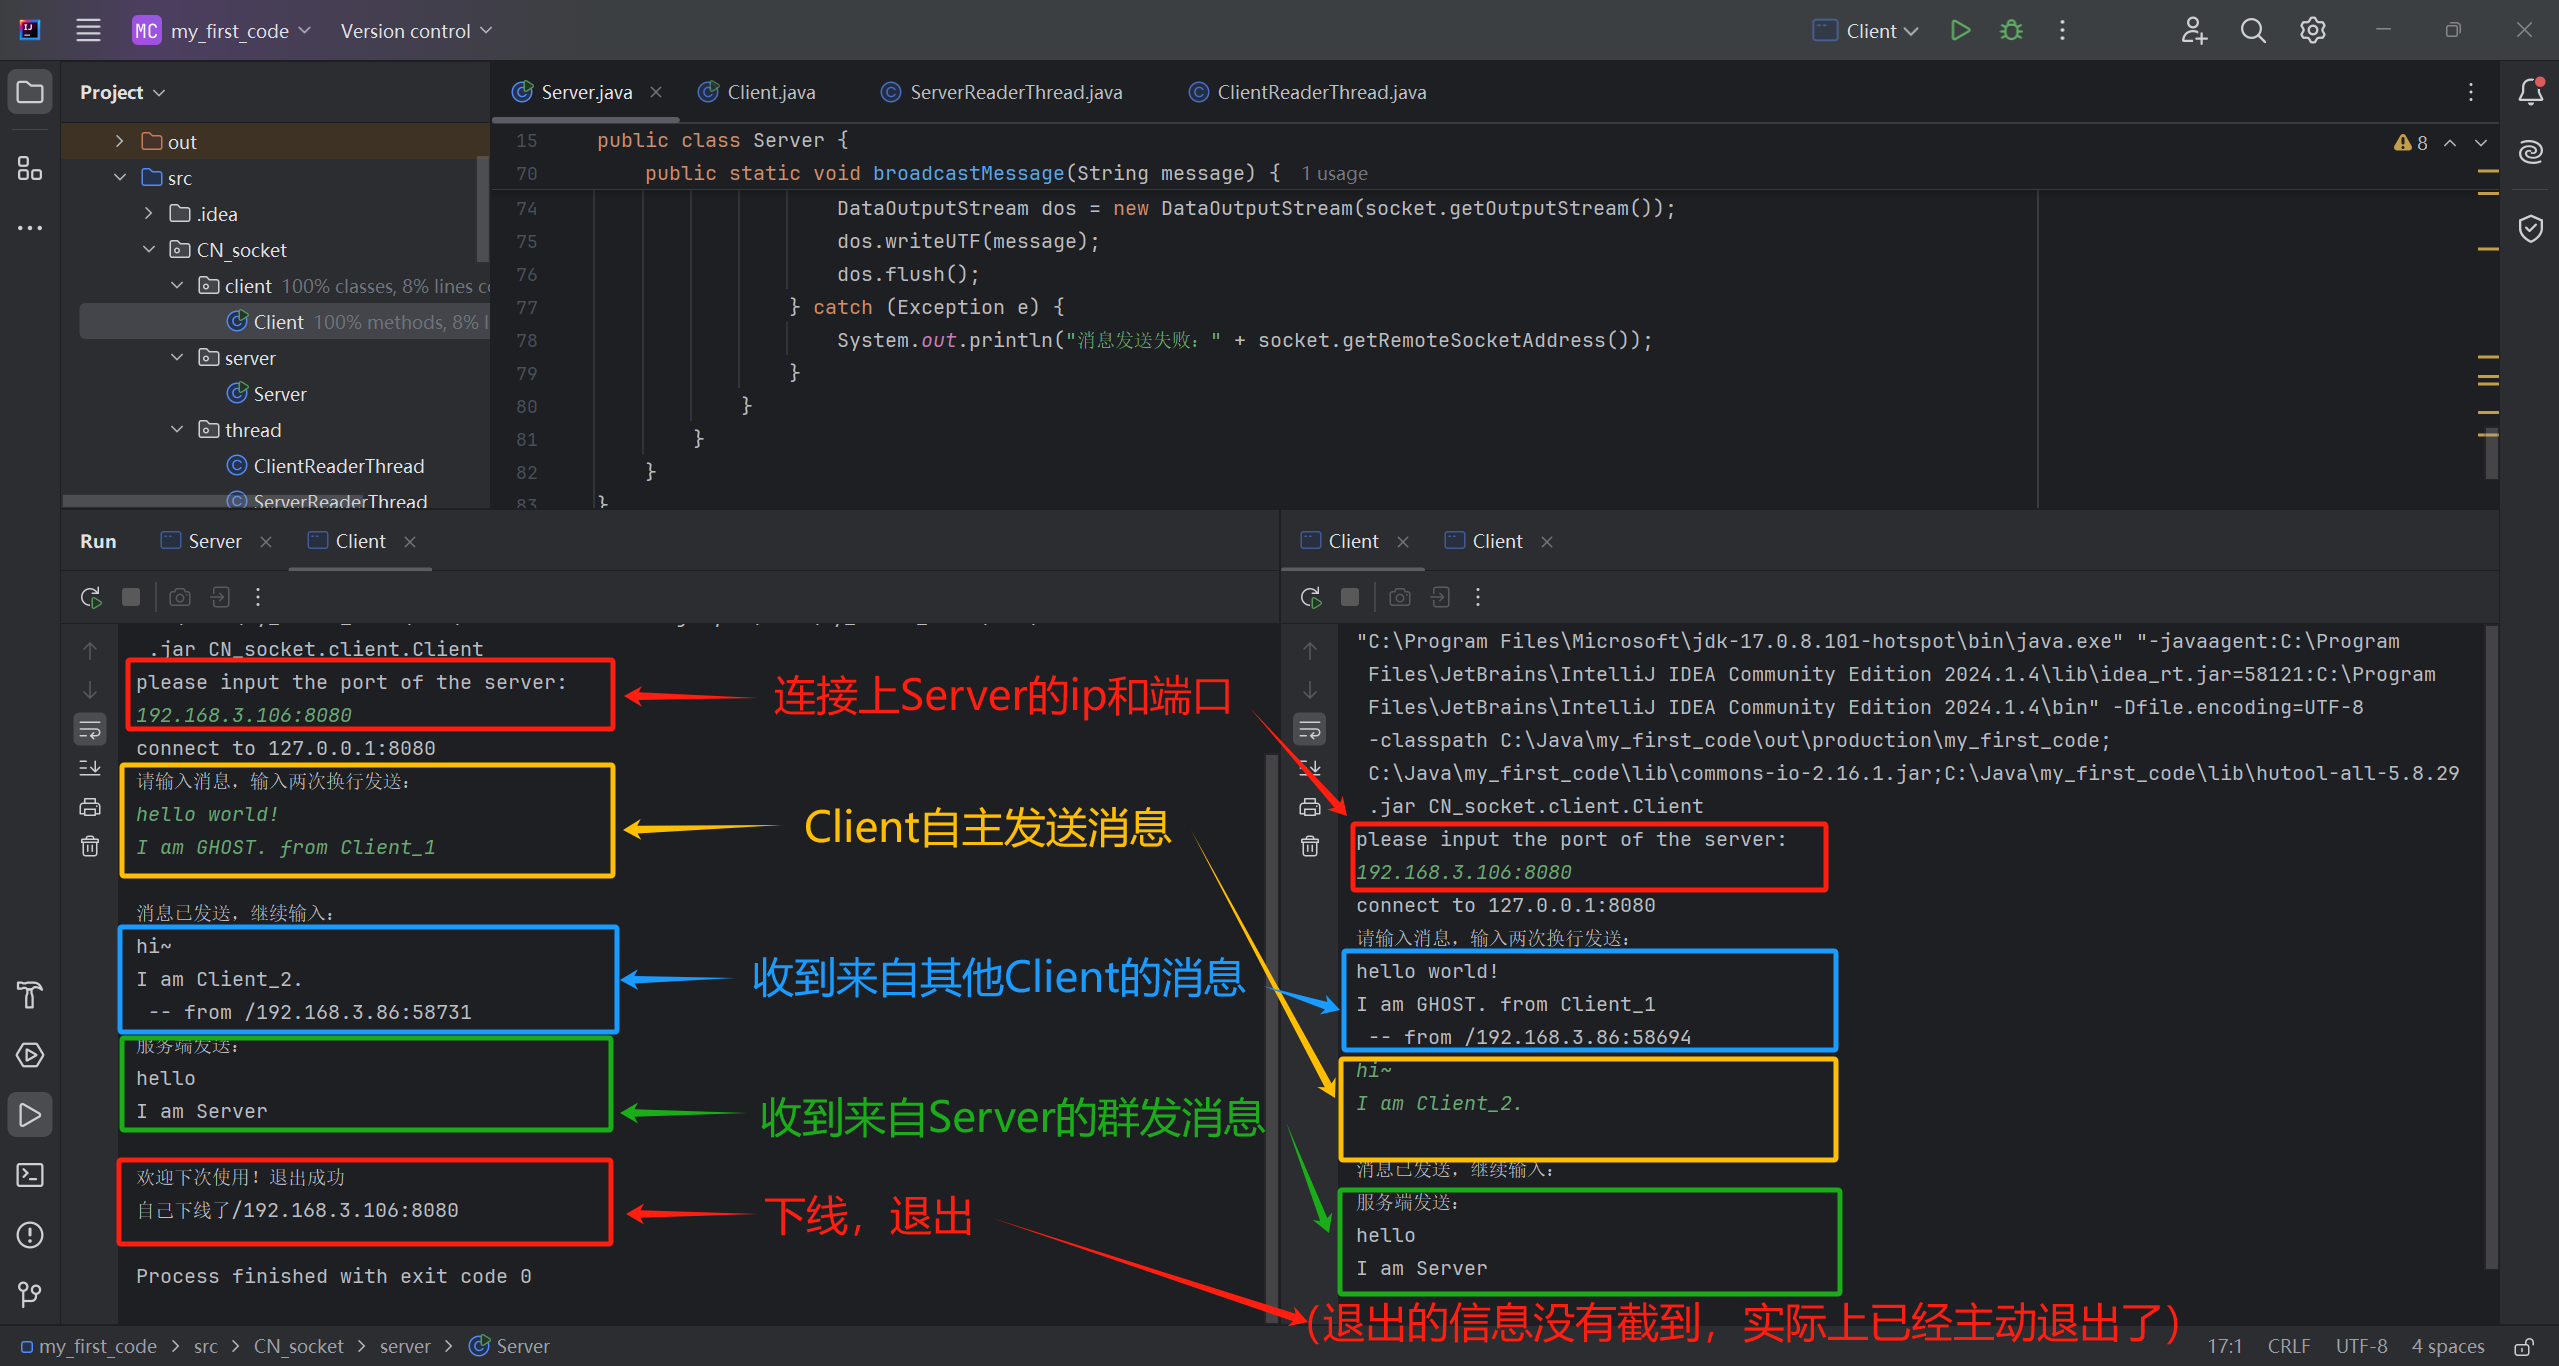
\includegraphics[width=15cm]{./images/7.支持在不同机器上通信-Client端.png}
		\caption{支持在不同机器上通信-Client端}
	\end{figure}
	
	\subsubsection{支持长文本消息(不少于20KB),有缓冲区管理}
	
	此处我使用了一个57.9KB的文件来上传,如下图所示。实验结果表面可以正常工作(且消息内容发送速度快,几乎无加载时长)
	
	\begin{figure}[H]
		\centering
		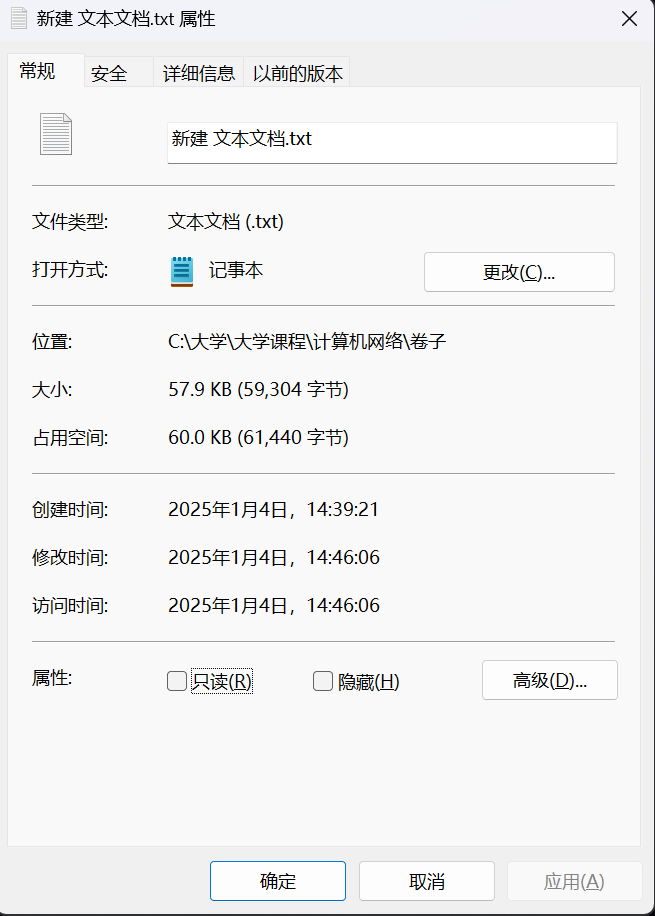
\includegraphics[width=6cm]{./images/8.该文本58KB.png}
		\caption{传输的文本大小为58KB}
	\end{figure}
	
	\begin{figure}[H]
		\centering
		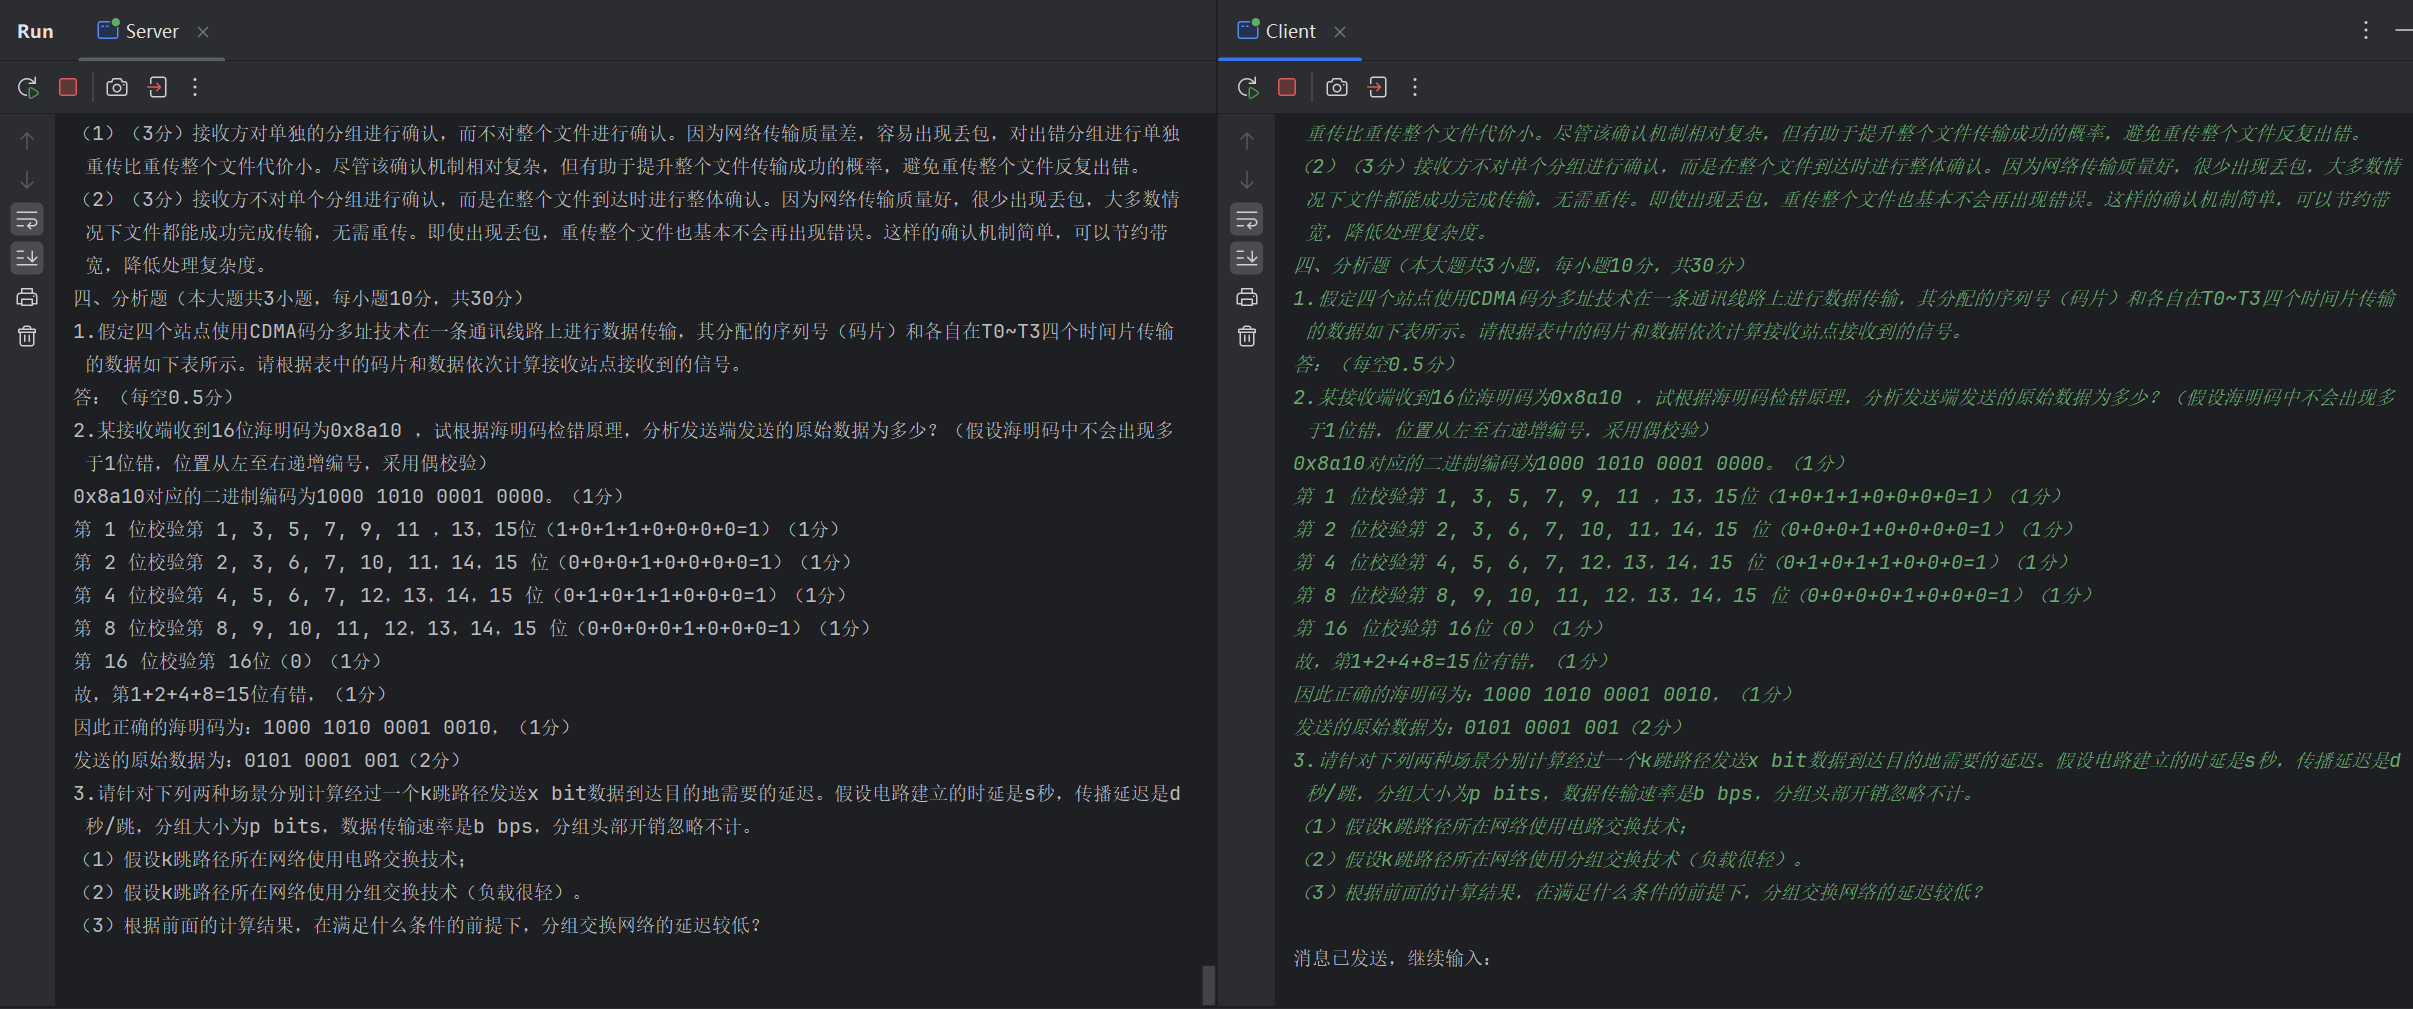
\includegraphics[width=15cm]{./images/8.支持长文本消息(该文本共58KB).png}
		\caption{支持长文本消息(该文本共58KB)}
	\end{figure}
	
	备注:左(Server)和右(Client)
	
	\subsubsection{容错性好,无闪退}
	
	从实验开始,截止到现在,所有的程序都可以正常工作,无闪退,容错性好。
	
	\subsection{Bonus}
	
	\subsubsection{支持双工通信}
	
	在server段开启一个线程发送消息即可。
	
	\begin{lstlisting}[language=Java, title=支持双工通信, tabsize=4]
	// Server.java
	StringBuilder messageBuffer = new StringBuilder();
	int emptyLineCount = 0;
	while (true) {
		String line = scanner.nextLine();
		if (line.trim().isEmpty()) {
			emptyLineCount++;
		} else {
			emptyLineCount = 0; // 重置计数
		}
		
		messageBuffer.append(line).append("\n");
		
		if (emptyLineCount == 1) {
			String message = messageBuffer.toString().trim(); // 去除多余的换行
			if (!message.isEmpty()) {
				broadcastMessage("服务端发送:\n" + message);
			}
			messageBuffer.setLength(0); // 清空缓冲区
			emptyLineCount = 0; // 重置计数
		}
	}
	\end{lstlisting}
	
	\begin{figure}[H]
		\centering
		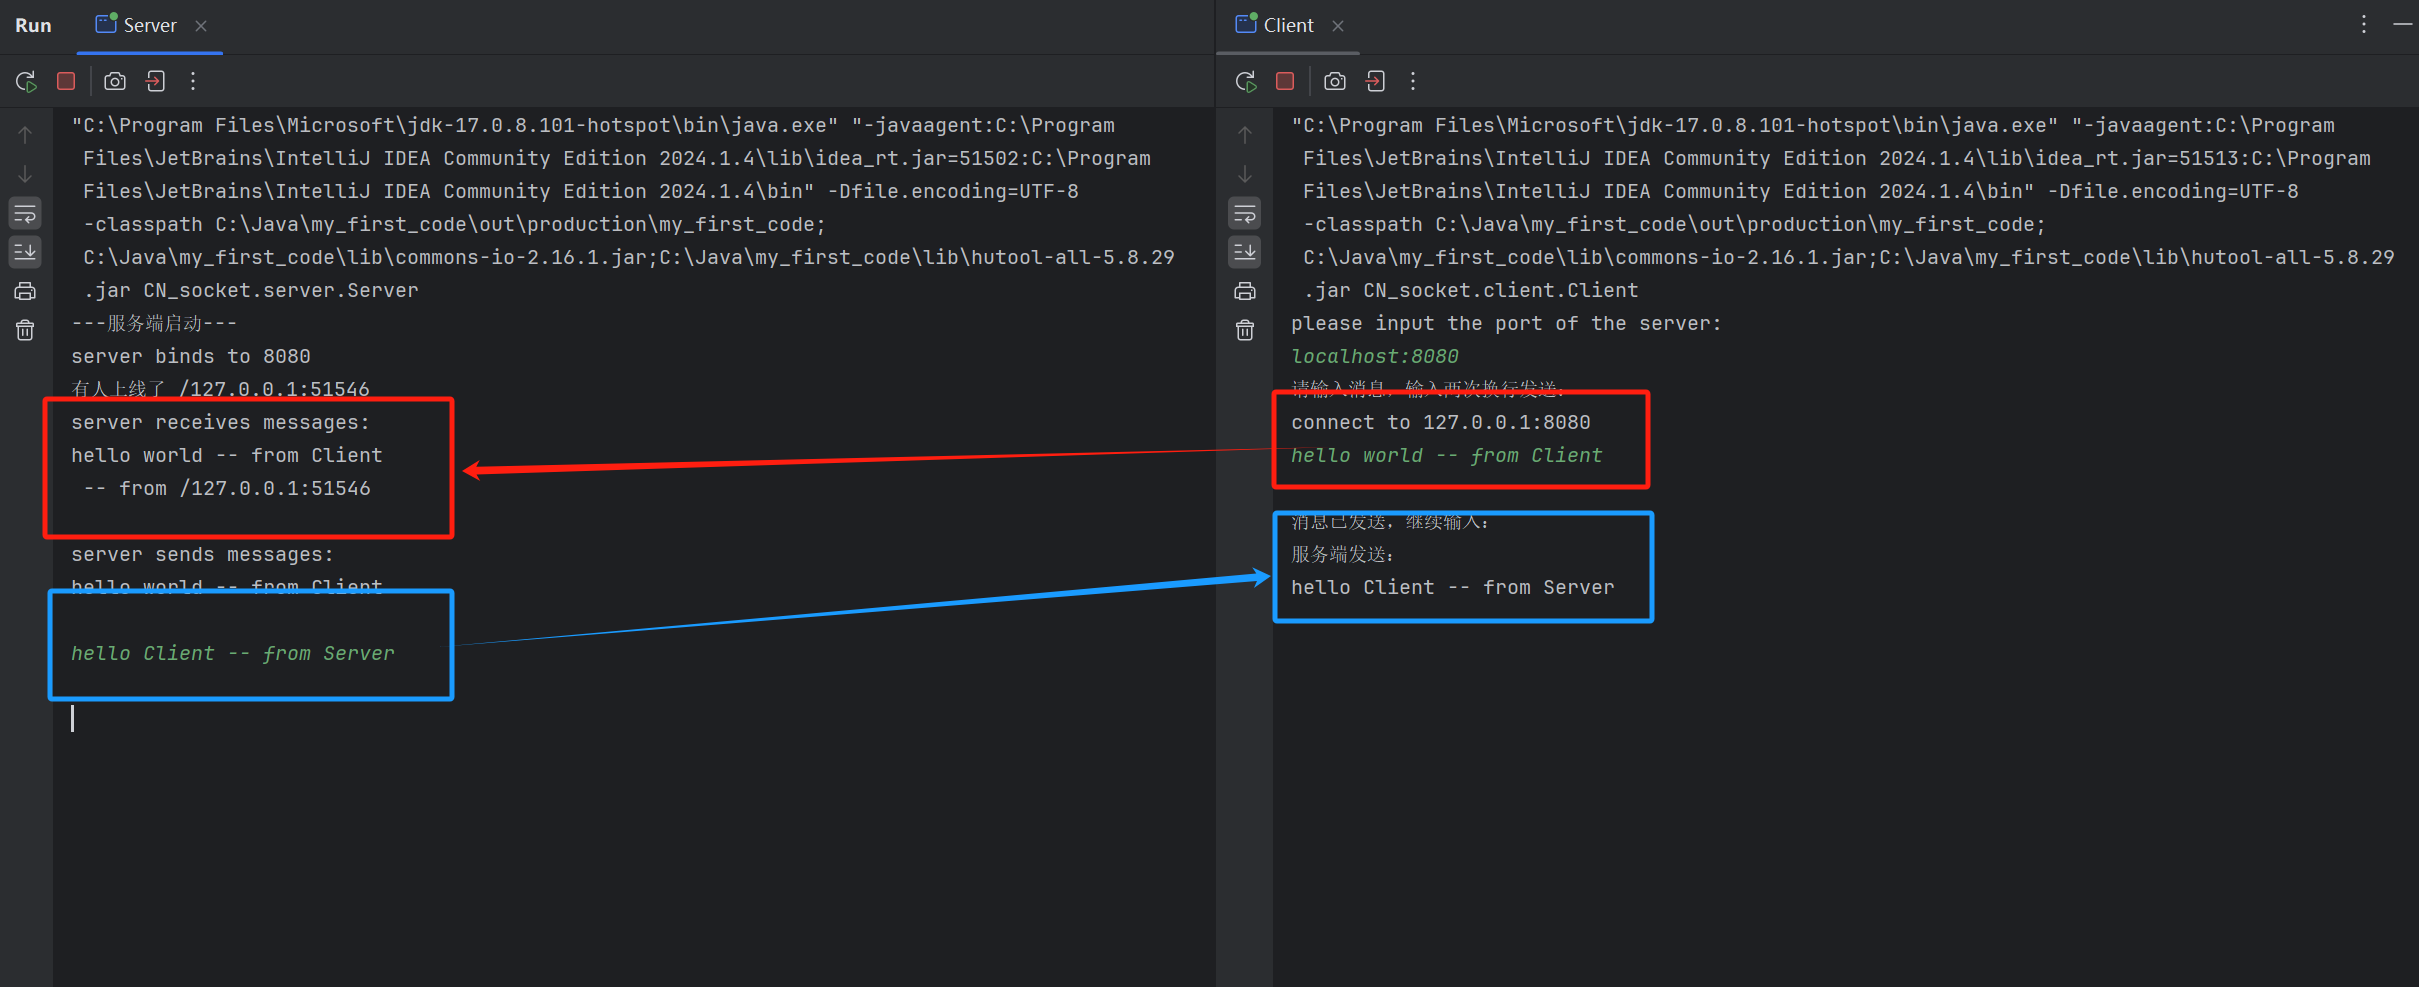
\includegraphics[width=15cm]{./images/9.支持双工通信.png}
		\caption{支持双工通信}
	\end{figure}
	
	备注:左(Server)和右(Client)
	
	\section{实验结果总结}
	
	至此,所有的测试和要求都已经通过,结果如下表所示:
	
	\begin{table}[!ht]
		\centering
		\begin{tabular}{|p{1.4cm}|p{1.4cm}|p{1.4cm}|p{1.4cm}|p{1.4cm}|p{1.4cm}|p{1.4cm}|p{1.4cm}|p{1.4cm}|p{1.4cm}|}
			\hline
			\multicolumn{3}{|c|}{server} & \multicolumn{3}{|c|}{client} & \multicolumn{3}{|c|}{整体} & 加分项 \\ \hline
			能在标准输出打印客户端发送的消息 & 支持5个以上客户端同时发送消息并主义打印 & 绑定至错误的端口号时能提示出错信息 & 能从标准输入或文件接收消息 & 标准输入消息以两次回车作为结束标志 & 连接至错误的IP地址/端口号时能提示出错信息 & 支持在localhost及在两台不同机器上运行 & 支持长文本消息(不少于20KB),有缓冲区管理 & 容错性好,无闪退 & 支持双工通信 \\ \hline
			完成 & 完成 & 完成 & 完成 & 完成 & 完成 & 完成 & 完成 & 完成 & 完成 \\ \hline
		\end{tabular}
	\end{table}
	
	通过本次实验,我深入学习了 Java 的网络编程,掌握了使用 Socket 进行客户端与服务端通信的核心技术,实现了消息的双工传输。实验过程中,我学会了如何设计多线程结构来处理多个客户端的并发连接,并通过合理的同步机制保证线程安全。此外,我还理解了网络编程中的基本概念,例如 IP 地址、端口号的配置以及网络通信协议的基本原理。同时,实验让我熟悉了使用 IntelliJ IDEA 进行项目开发的流程, 提高了调试和问题解决的能力。通过这次实践,我不仅巩固了 Java 基础,还加深了对网络编程应用场景的理解,为日后在分布式系统或实时通信领域的进一步学习奠定了基础。
	
	\section{附录}
	
	\subsection{说明}
	
	由于代码篇幅较长,我将已经完善的代码放在了GitHub仓库;
	
	可以访问:\texttt{https://github.com/SoftGhostGU/CodeExplorer}。
	
	以下是我的代码的结构和代码的具体内容。
	
	\subsection{代码结构}
	
	\begin{lstlisting}[numbers=none]
    CN_socket
    |-- README.md
    |-- src
    |   |-- CN_socket
    |   |   |-- client
    |   |   |   `-- Client.java
    |   |   |-- server
    |   |   |   `-- Server.java
    |   |   `-- thread
    |   |       |-- ClientReaderThread.java
    |   |       `-- ServerReaderThread.java
    `-- build
        `-- artifacts
        |-- client
        |   `-- client.jar
        `-- server
            `-- server.jar
    
    4 directories, 8 files
	\end{lstlisting}
	
	\subsection{源代码}
	
	\subsubsection{Client.java}
	
	\begin{lstlisting}[language=Java, title=Client.java, tabsize=4]
    package CN_socket.client;
    
    import CN_socket.thread.ClientReaderThread;
    
    import java.io.DataOutputStream;
    import java.io.OutputStream;
    import java.net.Socket;
    import java.util.Scanner;
    
    public class Client {
        public static void main(String[] args) throws Exception {
            Scanner sc = new Scanner(System.in);
            // 提示用户输入服务器地址和端口号
            System.out.println("please input the port of the server: ");
            String address_ = sc.nextLine();
            String address = address_.split(":")[0];
            int port_ = Integer.parseInt(address_.split(":")[1]);
            int port = 0;
            
            try {
            	// address 是用户输入的 IP 地址,port_ 是用户输入的端口号
            	if (port_ > 0 && port_ < 65535) {
            		port = port_;
            		
            		// 创建 Socket 对象,请求连接到指定服务器
            		Socket socket = new Socket(address, port);
            		
            		// 创建一个独立的线程,用于接收服务器发送的消息
            		new ClientReaderThread(socket).start();
            		
            		// 从 Socket 的输出流中获取字节输出流,用于向服务器发送消息
            		OutputStream os = socket.getOutputStream();
            		DataOutputStream dos = new DataOutputStream(os);
            		
            		// 用户输入消息并发送到服务器
            		Scanner scanner = new Scanner(System.in);
            		System.out.println("请输入消息,输入两次换行发送:");
            		StringBuilder messageBuilder = new StringBuilder();
            		while (true) {
            			String line = scanner.nextLine();
            			if (line.isEmpty()) {
            				// 检测到双换行,发送消息
            				String message = messageBuilder.toString();
            				if (message.trim().isEmpty()) {
            					System.out.println("欢迎下次使用!退出成功");
            					dos.close();
            					socket.close();
            					break;
            				}
            				dos.writeUTF(message); // 发送消息
            				dos.flush(); // 刷新输出流
            				messageBuilder.setLength(0); // 清空缓冲区
            				System.out.println("消息已发送,继续输入:");
            			} else {
            				// 累积消息内容
            				messageBuilder.append(line).append("\n");
            			}
            		}
            	} else {
            		throw new IllegalArgumentException("Invalid port: " + port_);
            	}
            } catch (IllegalArgumentException e) {
            	System.err.println("Wrong input: " + e.getMessage());
            } catch (Exception e) {
            	e.printStackTrace();
            }
    	}
    }
	\end{lstlisting}
	
	\subsubsection{Server.java}
	
	\begin{lstlisting}[language=Java, title=Server.java, tabsize=4]
	package CN_socket.server;
	
	import CN_socket.thread.ClientReaderThread;
	import CN_socket.thread.ServerReaderThread;
	
	import java.io.*;
	import java.net.InetAddress;
	import java.util.*;
	import java.net.BindException;
	import java.net.ServerSocket;
	import java.net.Socket;
	import java.util.ArrayList;
	import java.util.List;
	
	public class Server {
		public static List<Socket> onLineSockets = new ArrayList<>();
		
		public static void main(String[] args) {
			System.out.println("---服务端启动---");
			int port = 8080;
			
			try {
				ServerSocket serverSocket = new ServerSocket(port, 50, InetAddress.getByName("0.0.0.0"));
				System.out.println("server binds to " + port);
				
				new Thread(() -> {
					try (Scanner scanner = new Scanner(System.in)) {
						StringBuilder messageBuffer = new StringBuilder();
						int emptyLineCount = 0;
						
						while (true) {
							String line = scanner.nextLine();
							if (line.trim().isEmpty()) {
								emptyLineCount++;
							} else {
								emptyLineCount = 0; // 重置计数
							}
							
							messageBuffer.append(line).append("\n");
							
							if (emptyLineCount == 1) {
								String message = messageBuffer.toString().trim(); // 去除多余的换行
								if (!message.isEmpty()) {
									broadcastMessage("服务端发送:\n" + message);
								}
								messageBuffer.setLength(0); // 清空缓冲区
								emptyLineCount = 0; // 重置计数
							}
						}
					} catch (Exception e) {
						e.printStackTrace();
					}
				}).start();
				
				// 接收客户端连接
				while (true) {
					Socket socket = serverSocket.accept();
					synchronized (onLineSockets) {
						onLineSockets.add(socket);
					}
					System.out.println("有人上线了 " + socket.getRemoteSocketAddress());
					new ServerReaderThread(socket).start();
				}
			} catch (Exception e) {
				e.printStackTrace();
			}
		}
		
		// 广播消息给所有在线客户端
		public static void broadcastMessage(String message) {
			synchronized (onLineSockets) {
				for (Socket socket : onLineSockets) {
					try {
						DataOutputStream dos = new DataOutputStream(socket.getOutputStream());
						dos.writeUTF(message);
						dos.flush();
					} catch (Exception e) {
						System.out.println("消息发送失败:" + socket.getRemoteSocketAddress());
					}
				}
			}
		}
	}
	
	\end{lstlisting}
	
	\subsubsection{ClientReaderThread.java}
	
	\begin{lstlisting}[language=Java, title=ClientReaderThread.java, tabsize=4]
	package CN_socket.thread;
	
	import CN_socket.server.Server;
	
	import java.io.DataInputStream;
	import java.io.InputStream;
	import java.net.Socket;
	import java.util.ArrayList;
	import java.util.List;
	
	public class ClientReaderThread extends Thread {
		private Socket socket;
		public ClientReaderThread(Socket socket) {
			this.socket = socket;
		}
		
		@Override
		public void run() {
			System.out.println("connect to 127.0.0.1:8080");
			InputStream is = null;
			try {
				is = socket.getInputStream();
				DataInputStream dis = new DataInputStream(is);
				while (true) {
					try {
						String message = dis.readUTF();
						System.out.println(message);
					} catch (Exception e) {
						System.out.println("自己下线了" + socket.getRemoteSocketAddress());
						dis.close();
						socket.close();
						break;
					}
				}
			} catch (Exception e) {
				throw new RuntimeException(e);
			}
		}
	}
	
	\end{lstlisting}
	
	\subsubsection{ServerReaderThread.java}
	
	\begin{lstlisting}[language=Java, title=ServerReaderThread.java, tabsize=4]
	package CN_socket.thread;
	
	import CN_socket.server.Server;
	
	import java.io.*;
	import java.net.Socket;
	
	public class ServerReaderThread extends Thread {
		private Socket socket;
		public ServerReaderThread(Socket socket) {
			this.socket = socket;
		}
		
		@Override
		public void run() {
			InputStream is = null;
			try {
				is = socket.getInputStream();
				DataInputStream dis = new DataInputStream(is);
				while (true) {
					try {
						String message = dis.readUTF();
						System.out.println("server receives messages: ");
						System.out.println(message + " -- from " + socket.getRemoteSocketAddress());
						System.out.println();
						// 发送给其他所有用户
						System.out.println("server sends messages: ");
						System.out.println(message);
						sendMsgToAll(message);
					} catch (Exception e) {
						System.out.println("有人下线了 " + socket.getRemoteSocketAddress());
						Server.onLineSockets.remove(socket);
						dis.close();
						socket.close();
						break;
					}
				}
			} catch (Exception e) {
				throw new RuntimeException(e);
			}
		}
		
		private void sendMsgToAll(String msg) throws IOException {
			// 发送给其他所有的socket
			for (Socket onLineSocket: Server.onLineSockets) {
				if (onLineSocket.equals(socket)) {
					continue;
				}
				OutputStream os = onLineSocket.getOutputStream();
				DataOutputStream dos = new DataOutputStream(os);
				dos.writeUTF(msg + " -- from " + socket.getRemoteSocketAddress());
				dos.flush();
			}
		}
	}
	
	\end{lstlisting}
\end{document}
